%%  Manuscript submission to Communications in Number Theory and Physics
%%  Source repository: https://github.com/photodoc1960/Riemann-quantum-graph
%%  Markdown source:   Primes_in_the_Wires_v3.md
%%
%%  Requires the CNTP LaTeX support files (ipart.cls, ipart-layout-main.sty,
%%  imsart-number.bst, imsart-nameyear.bst) from
%%  https://github.com/vtex-soft/texsupport.intlpress-cntp
%%
%%  Pre-submission TODO for the author:
%%   1. Fill in MathSciNet IDs in the bibliography (search MathSciNet by title)
%%   2. Verify potential referee emails (see cover letter)
%%   3. Confirm author email and affiliation on title page
%%   4. Compile with pdflatex; review the typeset PDF before submission

\documentclass[cntp]{ipart}

\RequirePackage{hyperref}
\RequirePackage{amsmath}
\RequirePackage{amssymb}
\RequirePackage{graphicx}
\RequirePackage{float}

\startlocaldefs
\theoremstyle{plain}
\newtheorem{thm}{Theorem}[section]
\newtheorem{cor}[thm]{Corollary}
\theoremstyle{remark}
\newtheorem{rem}[thm]{Remark}
\endlocaldefs

%%  Filled by editor on acceptance
\pubyear{2026}
\volume{0}
\issue{0}
\firstpage{1}
\lastpage{1}
%\arxiv{}

\begin{document}

\begin{frontmatter}

\title[Vertex Boundary Conditions in Quantum Graphs]{Vertex Boundary Conditions Determine Spectral Correspondence in Quantum Graphs: Evidence for a Riemann-Specific Construction}

\begin{aug}
    \author{\fnms{J. D.} \snm{Slater}\ead[label=e1]{jdslater@colostate.edu}}
    \address{Department of Computer Science\\
             Colorado State University\\
             Fort Collins, CO 80523, USA\\
             and MERLN LLC\\
             Irving, TX 75038, USA\\
             \printead{e1}}
\end{aug}

\begin{abstract}
We measure spectral correspondence by a composite score $\mathcal{S} \in [0, 1]$ (higher is better; weighted from positional accuracy, GUE-spacing statistics, and pair correlation) and by the mean absolute deviation MAD of matched eigenvalue--target residuals, reported in units of the local mean zero spacing (``mean spacings''). Under standard Neumann boundary conditions, the cycle graph $C_n$ is spectrally equivalent to a single circle of circumference $L = \sum_e l_e$ with spectrum $k_m = 2\pi m / L$, independent of $n$; the correspondence score against any target collapses to a one-parameter family in $L$ (Theorem~\ref{thm:neumann}). Per-vertex TRS-breaking phases, which preserve reflectionlessness, enlarge this to a two-parameter family $(L, \Phi)$ with empirical ceiling $\mathcal{S} \approx 0.72$ at $N = 100$ Riemann zeros. Replacing Neumann with general U(2) vertex scattering, in which the reflection amplitude $|\cos\theta_v|$ becomes free, breaks this ceiling: the identical CMA-ES + Nelder--Mead pipeline reproducibly reaches MAD $= 0.148 \pm 0.006$ mean spacings on $C_7$ across $K_R = 30$ independent restart seeds (best single value $0.097$ observed on $C_{20}$ at a narrow local optimum; Section~\ref{sec:results-scaling}). Replacing the cycle by a theta graph at matched parameter count yields correspondence within $\pm 0.01$ in best-of-restart $\mathcal{S}$ across the tested parameter counts up to $96$ dimensions, indicating that the relevant degree of freedom is the dimension of the vertex unitary group, not the graph topology. The same pipeline against $K = 50$ independent GUE surrogate targets unfolded to the Riemann--von Mangoldt smooth density yields MAD $= 0.260 \pm 0.036$ mean spacings, with no overlap between the Riemann-seed and surrogate distributions (Cliff's $|\delta| = 1.000$; two-sided Mann--Whitney $U = 0$, exact $p \approx 2.3 \times 10^{-22}$). A reflection-magnitude ablation at fixed $\theta_v$ with the remaining three U(2) phases per vertex freely optimized yields an inverted-U curve peaking at $|\cos\theta_v| \approx 0.55$ with $\mathcal{S} = 0.886$; both the fully-reflecting and reflectionless extremes collapse to $\mathcal{S} \approx 0.73$, confirming the reflection-magnitude mechanism of Remark~\ref{rem:reflection} while identifying an optimal reflection amplitude in the middle of its range. The construction is not a generic GUE-density fitter; it finds structure specific to the Riemann zeros.
\end{abstract}

\begin{keyword}[class=MSC]
\kwdgroup[type=primary]{\kwd{81Q35}\kwd{11M26}}
\kwdgroup[type=secondary]{\kwd{34B45}\kwd{65F15}}
\end{keyword}

\begin{keyword}
\kwd{Quantum Graph}
\kwd{Spectral Correspondence}
\kwd{Riemann Zeros}
\kwd{Hilbert--P\'olya Conjecture}
\kwd{Vertex Boundary Conditions}
\end{keyword}

\end{frontmatter}

%% =====================================================================
\section{Introduction}
\label{sec:intro}

The spectral correspondence problem on a quantum graph asks: given a target sequence $\{\gamma_n\}$ of real numbers and a quantum graph $G$ with adjustable edge lengths and vertex boundary conditions, how closely can the eigenvalues $\{k_j\}$ of the self-adjoint graph Laplacian on $G$ approximate the targets? The problem is well-posed for any choice of $G$ and target sequence, and admits a natural quantitative score based on the positional accuracy of matched eigenvalue--target pairs after density normalization.

When $G$ is the cycle graph $C_n$ and the targets are the imaginary parts of the nontrivial zeros of the Riemann zeta function, the question acquires additional motivation from the Hilbert--P\'olya program. The conjecture posits that the zeros are eigenvalues of an undiscovered self-adjoint operator, with empirical support from the Montgomery--Odlyzko correspondence between zero statistics and the Gaussian Unitary Ensemble~\cite{r1,r2}. Quantum graphs are natural candidates because they admit self-adjoint extensions parameterized by unitary vertex scattering matrices~\cite{r3}, generically exhibit GUE spectral statistics~\cite{r4}, and possess trace formulas structurally parallel to Riemann's explicit formula~\cite{r5}. The Riemann zeros thus serve as both a mathematically natural target for the spectral correspondence problem and a connection point to a famous unsolved question.

We approach the spectral correspondence problem computationally: we optimize over edge lengths and vertex scattering parameters using covariance-matrix adaptation, score the resulting spectra against the first $N = 100$ Riemann zeros, and ask what the achievable scores reveal about which graph degrees of freedom matter. Four findings emerge.

\smallskip\noindent\textbf{First.} Neumann scattering on cycle graphs admits a hard correspondence ceiling that no edge-length variation or graph-size scaling can break. The mechanism is the spectral removability of degree-2 Kirchhoff vertices: under standard Neumann conditions, a degree-2 vertex imposes no constraint on a $C^1$ wavefunction, so $C_n$ with edge lengths $l_1, \ldots, l_n$ is isometric (as a metric space carrying $-d^2/dx^2$) to a single circle of circumference $L = \sum_e l_e$. The spectrum is therefore $k_m = 2\pi m / L$ for $m \in \mathbb{Z}_{\geq 0}$, independent of $n$ and of the partition of $L$ among edges, and the correspondence score reduces to a single continuous parameter $L$; for the first $100$ Riemann zeros, the maximum over $L$ is $\mathcal{S} \approx 0.092$. Adding per-vertex time-reversal-breaking phases (the conjugation $D_v \sigma_x D_v^\dagger$) keeps the scattering reflectionless and enlarges the parameter family to $(L, \Phi)$ with $\Phi = \sum_v \theta_v$; the empirical ceiling under this two-parameter family rises to $\mathcal{S} \approx 0.72$. Both ceilings are confirmed by exhaustive enumeration of $457$ of $853$ connected $7$-vertex graphs and by scaling measurements from $C_3$ through $C_{28}$. The constraining property in both cases is the reflectionlessness ($S_{ii} = 0$) of the degree-2 Neumann scattering matrix, not unitarity per se.

\smallskip\noindent\textbf{Second.} Replacing Neumann scattering with general U(2) vertex conditions breaks this ceiling decisively. The same $C_7$ topology under U(2) scattering reaches $\mathcal{S} = 0.897$ against $100$ Riemann zeros, with mean absolute deviation $0.145$ mean spacings (best of $30$ restarts, mean $0.884 \pm 0.006$). Across cycle sizes $C_5$ through $C_{21}$, the mean correspondence improves with $n$ at fixed optimization budget, reaching mean $0.907 \pm 0.010$ at $C_{20}$ and a verified best of $0.9258$ at MAD $= 0.097$ mean spacings --- the latter representing a narrow local optimum not reproducible from independent random initialization, but reproducible bit-exactly from the saved parameters. The improvement over the Neumann ceiling is the largest single-step effect observed in this study.

\smallskip\noindent\textbf{Third.} The spectral correspondence is approximately topology-independent at fixed parameter count. Replacing $C_n$ by a theta graph with two degree-3 hub vertices under U(3) scattering and degree-2 internal vertices under U(2) scattering --- varying the path length to match the cycle parameter count --- yields best-of-restart scores within $\pm 0.01$ of the matched cycle at every tested parameter count up to $96$ dimensions (mean-of-restarts differences $\pm 0.005$). The unitary group dimension at vertices is the relevant axis; the graph topology supporting them is not.

\smallskip\noindent\textbf{Fourth.} A direct distributional surrogate control establishes that the U(2) construction is not a generic capacity to fit GUE-distributed targets but instead finds structure specific to the Riemann zeros. Under $K_R = 30$ independent seeds of the identical CMA-ES + Nelder--Mead pipeline against the Riemann zeros, the resulting MAD distribution concentrates at $0.148 \pm 0.006$ mean spacings; the same pipeline against $K = 50$ independent GUE surrogate target sequences unfolded to the Riemann--von Mangoldt smooth counting density yields MAD $= 0.260 \pm 0.036$ mean spacings. The two distributions are disjoint (the Riemann maximum $0.159$ lies below the surrogate minimum $0.206$), with Cliff's $|\delta| = 1.000$ and a two-sided Mann--Whitney $U = 0$, exact $p \approx 2.3 \times 10^{-22}$. Every optimization on both sides matches all $100$ targets within the $\pm \Delta\gamma$ matching window, so the two MAD distributions are computed on a common denominator and the separation is carried entirely by positional accuracy on the matched targets, not by asymmetric coverage. A complementary reflection-magnitude ablation --- fixing $|\cos\theta_v|$ at every vertex and freely optimizing the remaining U(2) phases and edge lengths --- produces an inverted-U curve peaking at $|\cos\theta_v| \approx 0.55$ with $\mathcal{S} = 0.886$ and collapsing to $\mathcal{S} \approx 0.73$ at both the reflectionless and fully-reflecting extremes. This confirms the mechanistic role of reflection identified in Remark~\ref{rem:reflection} while identifying a specific optimal reflection amplitude in the interior of its range.

These results frame the spectral correspondence problem differently than the existing literature on quantum-graph approaches to the Riemann zeros, which has typically searched for special edge-length sequences (e.g., logarithms of primes) under fixed boundary conditions~\cite{r5,r8}. We find that edge geometry is not the carrier of the arithmetic information: the relevant freedom lives at the vertices, in the choice of self-adjoint extension. The Hilbert--P\'olya implications are suggestive but speculative. The U(2) vertex matrices we find are numerically generic --- a PSLQ integer-relation search at $50$ decimal places against bases of $\pi$, logarithms of primes up to $61$, and standard algebraic constants returns no relations with coefficients $|c| \leq 10$ at residuals below $10^{-20}$ --- so we cannot offer an analytic characterization of the optimal scattering data. We do not claim convergence of the finite quantum graph spectra to the actual Riemann zeros in the $n \to \infty$ limit, only an empirical improvement at the cycle sizes accessible to our optimization. What the results establish is that self-adjoint quantum-graph constructions exist whose first $100$ eigenvalues approximate the Riemann zeros to within $\sim 10\%$ of mean spacing, a quantitative numerical benchmark we believe to be novel for this construction class; that the relevant degree of freedom is the vertex boundary condition rather than the graph geometry; and that the construction finds structure specific to the Riemann zeros rather than to generic GUE-density targets.

%% =====================================================================
\section{Methods}
\label{sec:methods}

\subsection{Quantum graph construction}
\label{sec:methods-construction}

We construct quantum graphs on cycle topologies $C_n$ and on theta graphs $\Theta_k$ consisting of two hub vertices connected by three paths of $k$ edges each. The metric structure assigns each edge $e$ a positive length $l_e$. The self-adjoint Laplacian on the graph is determined by the choice of vertex scattering matrices $\{S_v\}$ subject to unitarity, with eigenvalues $k_j > 0$ given by solutions of the secular equation
\begin{equation}
    \det\bigl[I - S \cdot U(k)\bigr] = 0,
\end{equation}
where $S$ is the $2|E| \times 2|E|$ block-diagonal scattering matrix assembled from the per-vertex $S_v$, $U(k) = \operatorname{diag}(e^{i k l_b})$ is the bond propagation matrix, and $b = 1, \ldots, 2|E|$ indexes directed bonds (each undirected edge $e$ contributing two directed bonds of equal length $l_e$)~\cite{r3}.

Eigenvalues are located numerically by the following three-stage procedure. First, the interval $[10^{-6}, k_{\max}]$ is uniformly sampled at $n_{\mathrm{points}}$ points $\{k_1, \ldots, k_{n_{\mathrm{points}}}\}$, where $k_{\max} = \max\bigl((N + 5)\pi / L, 10\bigr)$ is set from the total graph length $L = \sum_e l_e$ and the number of target eigenvalues $N$; the additive $+5$ margin guards against boundary truncation. Optimization runs use $n_{\mathrm{points}} = 3000$; verification runs use $n_{\mathrm{points}} = 8000$ (Section~\ref{sec:methods-verify}). Second, the modulus $f(k) = |\det[I - S \cdot U(k)]|$ is evaluated at every sampled $k_i$ and a candidate eigenvalue is declared at every strict three-point interior minimum, i.e.\ every index $i$ with $f(k_i) < f(k_{i-1})$ and $f(k_i) < f(k_{i+1})$. Third, each candidate is refined by bounded Brent minimization (SciPy's \texttt{minimize\_scalar} with \texttt{method="bounded"}) of the same scalar $f(k)$ over the bracket $[k_{i-1}, k_{i+1}]$, and the refined minimum is accepted as an eigenvalue if $f$ at the refined point is below an acceptance threshold of $10^{-4}$. The refined eigenvalues are returned as a sorted list; the three-point strict-interior-minimum rule provides implicit de-duplication (adjacent samples cannot both be minima). We do not solve $\det = 0$ directly because $|{\det}|$ is a smooth non-negative function whose interior minima at true eigenvalues are quadratic in shape, while the complex-valued determinant crosses zero and its argument is numerically ill-conditioned near the eigenvalues.

\subsection{Scoring}
\label{sec:methods-scoring}

To compare graph eigenvalues $\{k_j\}$ against the first $N$ nontrivial zeros $\{\gamma_n\}$ of $\zeta(\tfrac{1}{2} + it)$, taken as the first $N$ imaginary parts $\gamma_n > 0$ computed to $50$ decimal places via mpmath's \texttt{zetazero} routine (arbitrary-precision arithmetic; more than sufficient given that all comparisons are made at eigenvalue spacings of order unity), we apply a nonlinear Weyl rescaling: each $k_j$ is mapped to
\begin{equation}
    T_j = N_{\mathrm{smooth}}^{-1}\!\left(\frac{L\,k_j}{\pi}\right),
\end{equation}
where $N_{\mathrm{smooth}}(T) = (T/2\pi)\ln(T/2\pi) - T/2\pi + 7/8$ is the Riemann--von Mangoldt smooth zero counting function and $L = \sum_e l_e$ is the total graph length. The inversion is performed pointwise via Brent's method applied to $N_{\mathrm{smooth}}(T) = L\,k_j/\pi$. This pointwise correction removes the systematic density mismatch between the uniform graph eigenvalue density $L/\pi$ and the logarithmic Riemann zero density $(2\pi)^{-1}\ln(T/2\pi)$ --- a correction that a linear rescaling cannot achieve~\cite{r8}. Rescaled eigenvalues $T_j$ falling within $\pm 1$ mean zero spacing of a target zero $\gamma_n$ form the comparison window; unmatched eigenvalues do not contribute to the score.

The total score is a fixed convex combination of three components,
\begin{equation}
    \mathcal{S} = 0.70\,\mathcal{S}_{\mathrm{pos}} + 0.20\,\mathcal{S}_{\mathrm{GUE}} + 0.10\,\mathcal{S}_{\mathrm{corr}},
\end{equation}
each normalized to $[0,1]$ with higher values indicating better correspondence. Denote the sequence of rescaled eigenvalues falling in the matching window by $\{T_j\}_{j=1}^{M}$ (in ascending order) and the matched target subsequence by $\{\gamma_{n_j}\}_{j=1}^{M}$, with $\Delta \gamma$ the mean nearest-neighbor spacing of $\{\gamma_n\}_{n=1}^{N}$. Then
\begin{equation}
    \mathcal{S}_{\mathrm{pos}} = \exp\!\left(-\,\frac{\mathrm{MAD}}{\Delta\gamma}\right), \qquad \mathrm{MAD} = \frac{1}{M}\sum_{j=1}^{M} \bigl|T_j - \gamma_{n_j}\bigr|,
\end{equation}
so an MAD of one mean spacing gives $\mathcal{S}_{\mathrm{pos}} = e^{-1} \approx 0.37$. Let $\{\tilde{k}_j\}$ denote the local polynomial unfolding of $\{T_j\}$ to unit mean density (degree $\min(5, \max(1, \lfloor M/10 \rfloor))$), $\{s_j\}$ its normalized nearest-neighbor spacings, and $F_{\mathrm{Wigner}}$ the cumulative distribution of the GUE Wigner surmise $P(s) = (32/\pi^2)\,s^2\,e^{-4s^2/\pi}$~\cite{r2}. Then
\begin{equation}
    \mathcal{S}_{\mathrm{GUE}} = \max\!\bigl(0,\,1 - D_{\mathrm{KS}}\bigr), \qquad D_{\mathrm{KS}} = \sup_s \bigl|\hat{F}_{\{s_j\}}(s) - F_{\mathrm{Wigner}}(s)\bigr|.
\end{equation}
Finally, let $\hat{R}_2(r)$ be the empirical two-point pair-correlation density of $\{\tilde{k}_j\}$ estimated as follows. Let $D = \{|\tilde{k}_i - \tilde{k}_j| : i < j,\ 0 < |\tilde{k}_i - \tilde{k}_j| \leq r_{\max}\}$ with $r_{\max} = 3$ (unordered pairs, self-pairs excluded). Bin $D$ uniformly into $n_b = 50$ bins on $(0, r_{\max}]$ of width $\Delta r = r_{\max}/n_b = 0.06$, taking $\hat{R}_2(r_b)$ as the density value at bin midpoint $r_b$ (histogram normalized to unit total mass over the domain). The GUE two-point correlation function is
\begin{equation}
    R_2^{\mathrm{GUE}}(r) = 1 - \left(\frac{\sin\pi r}{\pi r}\right)^2,
\end{equation}
which we discretize on the same $\{r_b\}$ grid and normalize by its own domain integral so that $\sum_b R_2^{\mathrm{GUE}}(r_b)\, \Delta r = 1$; this equalizes the two densities for comparison and removes any dependence on $r_{\max}$. Then
\begin{equation}
    \mathcal{S}_{\mathrm{corr}} = \exp\!\left(-\sum_b \bigl(\hat{R}_2(r_b) - R_2^{\mathrm{GUE}}(r_b)\bigr)^2 \Delta r\right).
\end{equation}
Scoring is validated against two reference cases at $N = 20$ zeros. Self-comparison (the first $20$ Riemann zeros scored against themselves) yields $\mathcal{S} = 0.955$, establishing the practical ceiling; the ceiling is bounded strictly below $1$ because $\mathcal{S}_{\mathrm{GUE}}$ and $\mathcal{S}_{\mathrm{corr}}$ take Kolmogorov--Smirnov and histogram-difference values that are positive at finite $N$ under the finite-size fluctuations of the Wigner surmise. The floor is calibrated against a null distribution of independently drawn uniform pseudo-eigenvalues: $50$ values sampled i.i.d.\ from $U(10, 250)$, sorted, and scored against the same $20$ Riemann targets. A single reference seed yields $\mathcal{S} = 0.144$; across $100$ independent seeds the null distribution is $\mathcal{S} = 0.21 \pm 0.09$ (mean $\pm$ standard deviation), median $0.19$, range $[0.05, 0.53]$, reflecting that individual realizations of a uniform null can occasionally place several pseudo-eigenvalues near Riemann targets. All optimized scores reported in this manuscript are well above the null tail: the pure-Neumann ceiling at $\mathcal{S} \approx 0.09$ is below even the null minimum (since Neumann on a cycle has only one degree of freedom while the null has $50$), and the U(2) results at $\mathcal{S} \approx 0.89$ are well above the null maximum.

The matching window is defined by $|T_j - \gamma_n| \leq \Delta\gamma$ and applied greedily in ascending order of $j$: eigenvalue $T_j$ is matched to the nearest as-yet-unmatched target zero within its window; eigenvalues whose window contains no unmatched target do not contribute. This produces a one-to-one, order-preserving pairing between a subset of $\{T_j\}$ and a subset of $\{\gamma_n\}$. The MAD in $\mathcal{S}_{\mathrm{pos}}$ is taken over matched pairs only; the matched count $M$ is reported alongside MAD for every comparison so that per-pair precision and coverage can be assessed jointly.

\subsection{Vertex scattering parameterizations}
\label{sec:methods-scattering}

We employ three families of vertex scattering matrices, of increasing generality.

\paragraph{Neumann.} The standard Neumann scattering matrix at a degree-$d$ vertex is $S_{ij} = 2/d - \delta_{ij}$. At degree 2 this reduces to the permutation $\sigma_x = \bigl(\begin{smallmatrix} 0 & 1 \\ 1 & 0 \end{smallmatrix}\bigr)$, which satisfies $\sigma_x^2 = I$.

\paragraph{TRS-broken Neumann.} A one-parameter extension introduces per-vertex time-reversal-breaking phases via the similarity transform $D_v\,S_v^{\mathrm{Neumann}}\,D_v^\dagger$ with $D_v = \operatorname{diag}(1, e^{i\theta_v}, \ldots, e^{i(d-1)\theta_v})$, preserving unitarity exactly.

\paragraph{Full U(d).} Every $d \times d$ unitary matrix $S_v$ corresponds to a self-adjoint boundary condition at a degree-$d$ vertex via the Kostrykin--Schrader parameterization $S_v = -(A + iB)^{-1}(A - iB)$ of self-adjoint extensions of the graph Laplacian~\cite{r3,r10}. We take each $S_v \in \mathrm{U}(d)$ to be \emph{$k$-independent}: the same unitary matrix appears in the secular equation~(1) at every wavenumber $k$. This is a $k$-independent slice through the full space of self-adjoint extensions (which in general admits $k$-dependent boundary conditions~\cite{r3}); we do not optimize over $k$-dependent extensions in this work. The resulting operator is self-adjoint by construction for every choice of the vertex parameters. For $d = 2$ we use the standard four-parameter form
\begin{equation}
    U_v = e^{i\alpha} \begin{pmatrix} e^{i\beta}\cos\theta & -e^{-i\gamma}\sin\theta \\ e^{i\gamma}\sin\theta & e^{-i\beta}\cos\theta \end{pmatrix}, \qquad \alpha, \beta, \gamma, \theta \in \mathbb{R},
\end{equation}
introducing 4 real degrees of freedom per vertex. For degree $d > 2$ we parameterize via the matrix exponential $U_v = \exp(iH_v)$ with $H_v$ a $d \times d$ Hermitian matrix specified by $d^2$ real parameters, giving 9 parameters per U(3) vertex.

\subsection{Optimization}
\label{sec:methods-opt}

{\sloppy Two black-box optimizers are used in this study. The exhaustive 7-vertex sweep (Section~\ref{sec:results-topology}) employs differential evolution (SciPy's \texttt{differential\_evolution} with the \texttt{best1bin} strategy, population size $15$, mutation $\in [0.5, 1.0]$, recombination $0.7$, and $10^4$ function evaluations per graph), chosen for throughput across $457$ graphs at moderate parameter dimension.\par} All remaining experiments (cycle scaling under Neumann, TRS-broken Neumann, and U(2) scattering; theta-graph comparison; U(3) extensions; and the surrogate control) use the covariance-matrix adaptation evolution strategy (CMA-ES~\cite{r11}, \texttt{cma} Python package version $3.3.0$) with population size $\lambda = 4 + \lfloor 3 \ln n_{\mathrm{param}} \rfloor$, initial step size $\sigma_0 = 0.5$, and a budget of $7.5 \times 10^4$ to $10^5$ function evaluations per restart. In both pipelines the black-box optimizer is followed by a Nelder--Mead local polish (SciPy, tolerance $10^{-8}$). The optimization objective is $1 - \mathcal{S}$. Restart counts vary by experiment: headline U(2) results on individual cycle graphs use $10$--$30$ independent restarts per graph; the surrogate control (Section~\ref{sec:results-surrogate}), the Riemann-seed distribution (Section~\ref{sec:results-surrogate}), and the reflection-magnitude ablation (Section~\ref{sec:results-reflection}) use $5$ restarts per experimental unit for parity across arms of those comparisons, so that each Riemann seed, each surrogate target, and each fixed-$\theta$ ablation point receives the same optimization budget. See Table~\ref{tab:experiment-map} for the per-experiment settings. All results reported represent the best solution found across the stated restarts, from uniformly random initializations. Edge lengths are bounded to $l_e \in [0.05, 5]$ throughout; no explicit scale-fixing constraint is imposed on $L = \sum_e l_e$ because the Weyl rescaling of Section~\ref{sec:methods-scoring} absorbs a global length rescaling into the map $k_j \mapsto T_j$, so $L$ is only a soft optimization variable rather than a physical unit choice.

\begin{table}[H]
\centering
\footnotesize
\begin{tabular}{@{}p{0.06\linewidth}p{0.34\linewidth}p{0.22\linewidth}p{0.10\linewidth}p{0.12\linewidth}@{}}
\hline
\S & Experiment & Scattering & Optimizer & Restarts \\
\hline
\ref{sec:results-topology} & $7$-vertex enumeration ($457$ graphs) & TRS-broken Neumann & DE & $1$ \\
\ref{sec:results-neumann} & Cycle $C_n$ Neumann ceiling & Pure Neumann & CMA-ES & $10$ \\
\ref{sec:results-neumann} & Cycle $C_n$ TRS-broken ceiling & TRS-broken Neumann & CMA-ES & $10$ \\
\ref{sec:results-U2} & $C_7$, cycle-size scaling $C_5$--$C_{21}$ & U(2) & CMA-ES & $10$--$30$ \\
\ref{sec:results-topology-indep} & Theta $\Theta_k$ topology & U(2), U(3) & CMA-ES & $10$ \\
\ref{sec:results-surrogate} & Riemann-seed distribution ($K_R=30$) & U(2) on $C_7$ & CMA-ES & $5$ / seed \\
\ref{sec:results-surrogate} & GUE surrogate control ($K=50$) & U(2) on $C_7$ & CMA-ES & $5$ / surrogate \\
\ref{sec:results-reflection} & Reflection ablation ($12$ $\theta$) & U(2) on $C_7$, fixed $\theta_v$ & CMA-ES & $5$ / $\theta$ \\
\hline
\end{tabular}
\caption{Mapping of manuscript experiments to graph family, scattering-matrix family, black-box optimizer, and CMA-ES restart count. All pipelines are followed by a Nelder--Mead polish. The three arms of the distribution/ablation comparison (Riemann-seed distribution, GUE surrogate control, reflection-magnitude ablation) use identical restart counts ($5$ per experimental unit) so that any observed distributional separation is not attributable to unequal compute.}
\label{tab:experiment-map}
\end{table}

\subsection{Verification protocol}
\label{sec:methods-verify}

The spectrum computation is sensitive to the secular determinant sampling resolution $n_{\mathrm{points}}$. Optimization runs use $n_{\mathrm{points}} = 3000$ for efficiency; reported headline scores are recomputed at $n_{\mathrm{points}} = 8000$ for resolution convergence, with score differences between resolutions typically below $0.0005$. Best-of-restart results are additionally verified by re-scoring the saved parameters from scratch in a separate Python process, confirming bit-exact reproducibility.

%% =====================================================================
\section{Results}
\label{sec:results}

\subsection{Topology search at 7 vertices}
\label{sec:results-topology}

We performed exhaustive enumeration of all $853$ non-isomorphic connected graphs on $7$ vertices, scored against the first $N = 20$ Riemann zeros (the reduced $N$ was used at this stage for throughput across $853$ candidates; all subsequent results in Sections~\ref{sec:results-neumann}--\ref{sec:results-surrogate} use $N = 100$). Of these, $457$ received full joint optimization over edge lengths and per-vertex TRS-breaking phases $\theta_v$ (Section~\ref{sec:methods-scattering}, ``TRS-broken Neumann'' family) via differential evolution; the remaining $396$, all having $12$ or more edges, were excluded after a preliminary screen. The preliminary screen ran the same differential-evolution pipeline with $10^3$ evaluations per graph (rather than the $10^4$ used for the full sweep) on a random subsample of $50$ of the excluded graphs distributed uniformly across the $12$--$21$ edge range; the maximum $\mathcal{S}$ observed in this screen was $0.53$. The exclusion is therefore an evidence-based extrapolation, not a proof: we cannot rule out that a graph with $\geq 12$ edges reaches $\mathcal{S} > 0.53$ under a larger evaluation budget, but the observed monotone decay with edge count (Figure~\ref{fig:scoreVsEdges}) makes this unlikely.

Under this TRS-broken Neumann scoring, the cycle $C_7$ achieves the highest score among the $457$ fully optimized graphs, $\mathcal{S} = 0.795$ (at $N = 20$), well above the second-best graph in the optimized subset (index $\#110$, degree sequence $[3,3,2,2,2,2,2]$, two independent cycles) at $\mathcal{S} = 0.762$. This value is consistent with the TRS-broken Neumann ceiling at $\mathcal{S} \approx 0.72$ measured at $N = 100$ (Corollary~\ref{cor:ceiling}, Remark~\ref{rem:trs}): scores at $N = 20$ are higher than at $N = 100$ because the two-parameter $(L, \Phi)$ family has more angular freedom relative to $20$ than to $100$ target constraints. Across the $457$ optimized graphs, scores distribute broadly (mean $0.486$, std $0.095$, median $0.485$) and correlate inversely with edge count (Pearson $r = -0.70$): every additional edge degrades the match (Figure~\ref{fig:scoreVsEdges}). The 7-edge and 8-edge graphs dominate the top 20; no graph with more than 10 edges exceeds $\mathcal{S} = 0.71$. Among the optimized graphs, $55$ exhibit three or more edges systematically driven to the optimizer's lower bound ($l_e < 0.05$), effectively collapsing the graph toward a simpler topology. This suggests the relevant spectral structure is carried by the minimal cycle, not by additional connectivity, and motivates focusing on cycle graphs $C_n$ for the remainder of the study.

\begin{figure}[H]
\centering
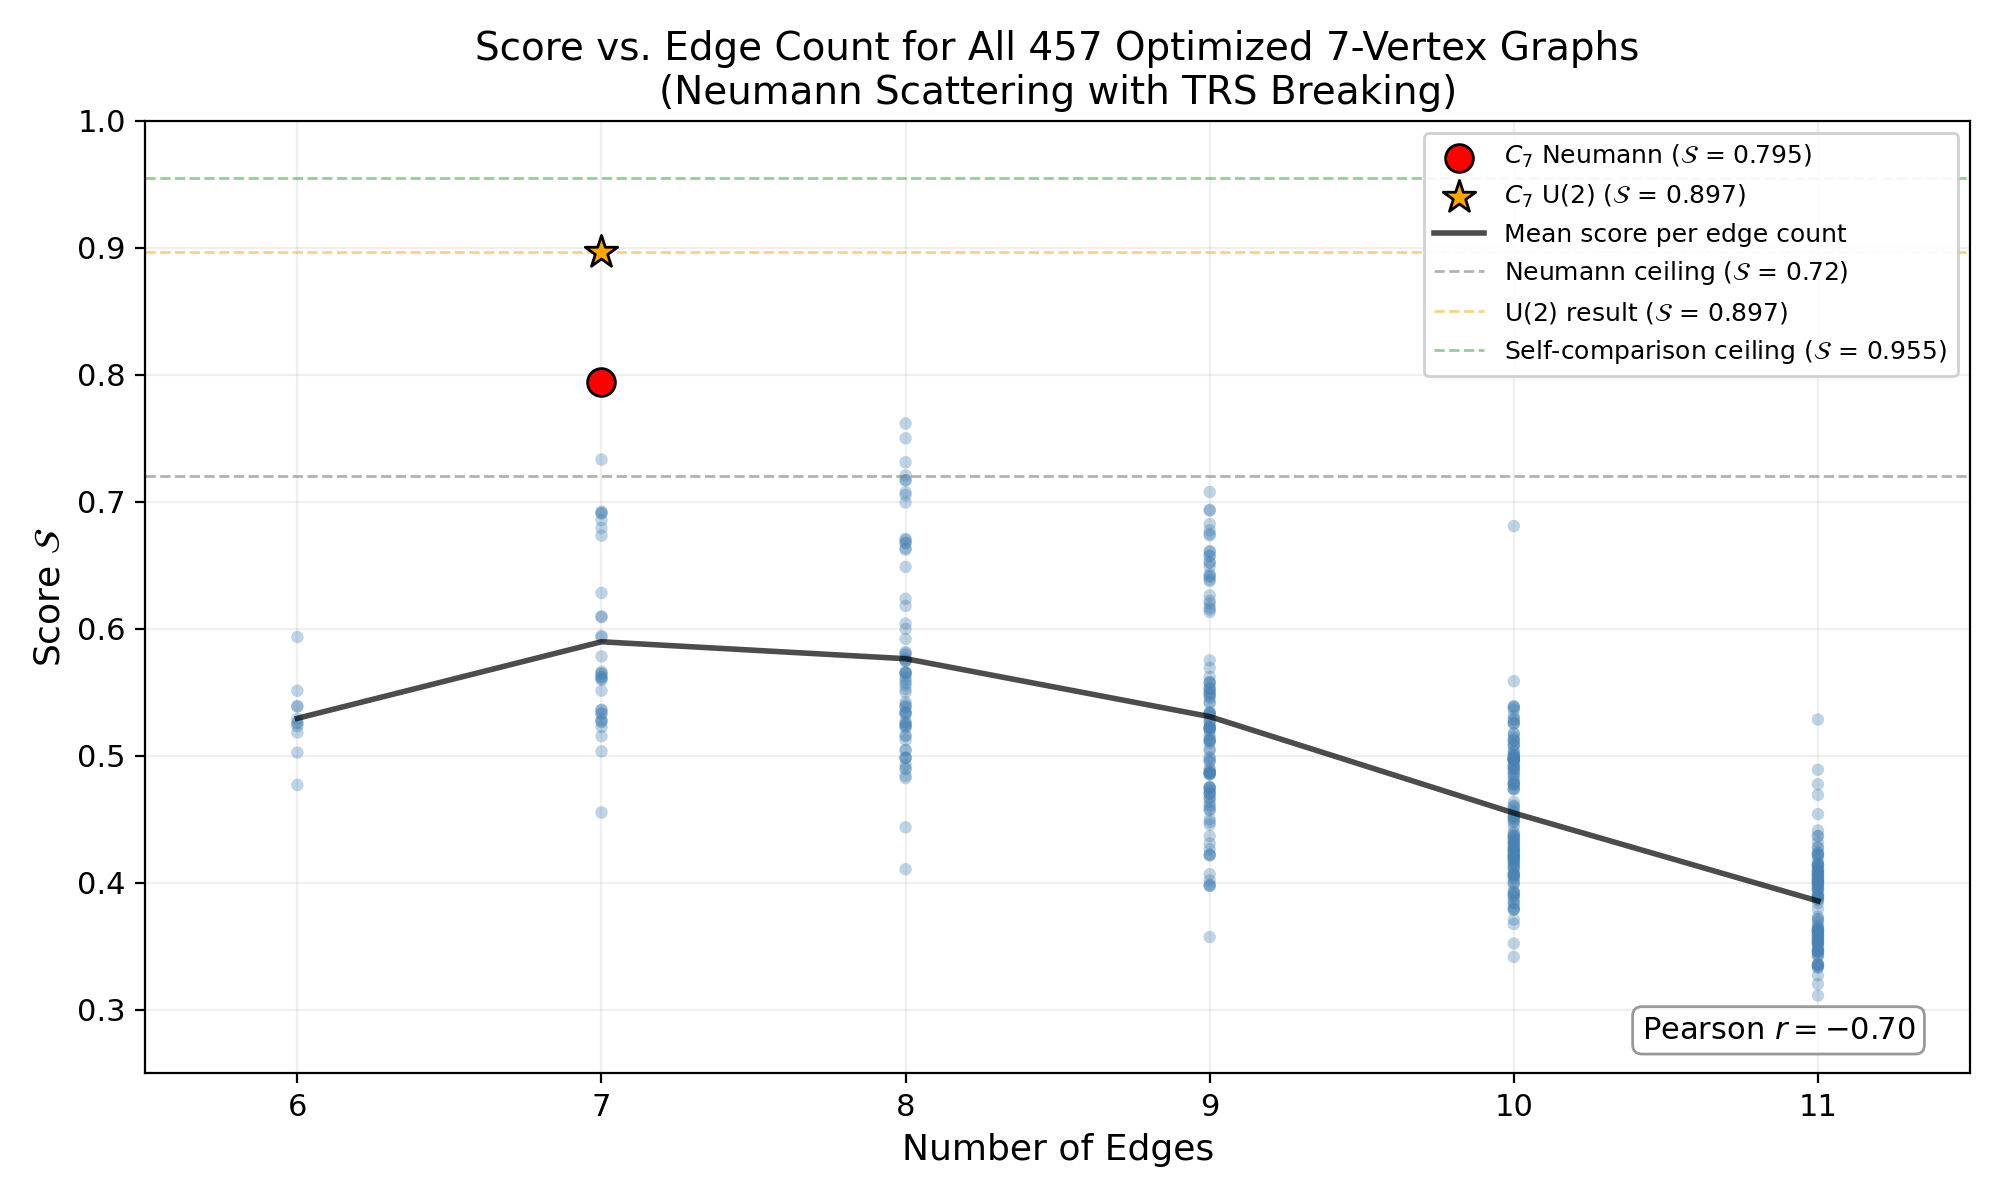
\includegraphics[width=\linewidth]{results/figure1_score_vs_edges.png}
\caption{Score versus edge count for all $457$ optimized $7$-vertex graphs under TRS-broken Neumann scattering, evaluated at $N = 20$ Riemann zeros (blue points). The cycle $C_7$ (red circle, $7$ edges) achieves the highest TRS-broken Neumann score $\mathcal{S} = 0.795$. Score correlates inversely with edge count (Pearson $r = -0.70$). The orange star shows $C_7$ under optimized U(2) vertex scattering (evaluated at $N = 100$, $\mathcal{S} = 0.897$), demonstrating that the same topology under general unitary vertex conditions breaks decisively through the TRS-broken Neumann ceiling. Dashed horizontal lines indicate the TRS-broken Neumann ceiling at $N = 100$ ($\mathcal{S} \approx 0.72$; Corollary~\ref{cor:ceiling}), the $C_7$ U(2) result at $N = 100$ ($\mathcal{S} = 0.897$), and the self-comparison ceiling at $N = 100$ ($\mathcal{S} = 0.955$). The pure-Neumann ceiling ($\mathcal{S} \approx 0.092$ at $N = 100$; Theorem~\ref{thm:neumann}) is not shown because pure-Neumann scattering was not used in the 7-vertex sweep.}
\label{fig:scoreVsEdges}
\end{figure}

\subsection{Neumann ceiling}
\label{sec:results-neumann}

We first establish the algebraic origin of the Neumann correspondence ceiling as a precise statement about the spectrum of $C_n$ under standard Neumann boundary conditions.

\begin{thm}[Neumann rigidity on cycle graphs]\label{thm:neumann}
Let $C_n$ denote the cycle graph on $n$ vertices with edge lengths $l_1, \ldots, l_n > 0$, and let the Laplacian on $C_n$ be equipped with standard Neumann (Kirchhoff) conditions at every degree-$2$ vertex. Then the spectrum of the resulting self-adjoint operator depends on the edge lengths only through their sum $L = \sum_{e=1}^{n} l_e$, and is
\begin{equation}
    k_m = \frac{2\pi m}{L}, \qquad m \in \mathbb{Z}_{\geq 0},
\end{equation}
with $k_0 = 0$ simple and each $k_m$ for $m \geq 1$ doubly degenerate. The spectrum is independent of the partition of $L$ among individual edges and of $n$, including its parity.
\end{thm}

\begin{proof}
At a degree-2 vertex the Kirchhoff conditions require continuity of $\psi$ and continuity of $\psi'$. These conditions impose no constraint on a $C^1$ function, so a degree-2 Kirchhoff vertex is spectrally removable~\cite{r10}. Hence $C_n$, viewed as a metric space carrying the operator $-d^2/dx^2$ on each edge, is isometric to a single circle of circumference $L = \sum_e l_e$. The Neumann graph Laplacian on $C_n$ is unitarily equivalent to the Laplacian on this circle with periodic boundary conditions, whose spectrum is $k_m = 2\pi m / L$ with the stated degeneracies.

Equivalently in the bond picture: the Neumann scattering matrix at a degree-2 vertex, $\sigma_x = \bigl(\begin{smallmatrix} 0 & 1 \\ 1 & 0 \end{smallmatrix}\bigr)$, is reflectionless ($S_{ii} = 0$). The bond-level scattering operator $S \cdot U(k)$ therefore decouples into two independent channels --- forward-traversing and backward-traversing bond eigenfunctions --- each of which is a weighted $n$-cycle whose monodromy reduces to the scalar $\prod_{v=1}^{n} e^{ik l_v} = e^{ikL}$. The eigenvalue condition $e^{ikL} = 1$ in each channel gives $k_m = 2\pi m / L$. The double degeneracy at $m \geq 1$ arises because forward and backward channels yield the same eigenvalues; the simple eigenvalue at $m = 0$ corresponds to the constant eigenfunction common to both channels.
\end{proof}

\begin{cor}[Neumann correspondence ceiling]\label{cor:ceiling}
Under Neumann boundary conditions, the spectrum of $C_n$ is a single arithmetic progression of spacing $2\pi / L$. The correspondence score $\mathcal{S}$ against any target sequence therefore depends on a single continuous parameter $L > 0$, independent of $n$. Numerical maximization of $\mathcal{S}$ over $L$ for the first $N = 100$ Riemann zeros under our scoring (Section~\ref{sec:methods-scoring}) yields $\mathcal{S}_{\mathrm{Neumann}}^{\max} \approx 0.092$, confirmed across $C_3$ through $C_{28}$ to a standard deviation $< 0.003$ (Figure~\ref{fig:neumannResiduals}).
\end{cor}

\begin{rem}[TRS-broken Neumann extension]\label{rem:trs}
Introducing per-vertex TRS-breaking phases via the similarity transform $D_v \sigma_x D_v^\dagger$ with $D_v = \operatorname{diag}(1, e^{i\theta_v})$ yields
\begin{equation}
    D_v \sigma_x D_v^\dagger = \begin{pmatrix} 0 & e^{-i\theta_v} \\ e^{i\theta_v} & 0 \end{pmatrix},
\end{equation}
which is still reflectionless (diagonal entries vanish): the conjugation introduces direction-dependent transmission phases but no reflection amplitude. The forward and backward channels remain decoupled and now accumulate opposite monodromy phases $\pm \Phi$ with $\Phi = \sum_v \theta_v$, so the spectrum splits into two interleaved uniform ladders
\begin{equation}
    k_m^{\pm} = \frac{2\pi m \pm \Phi}{L}, \qquad m \in \mathbb{Z}_{\geq 0}.
\end{equation}
The TRS-broken Neumann spectrum is therefore a two-parameter rigid family $(L, \Phi)$, with the achievable set identical for every $n$: $L$ ranges over $(0, \infty)$ and $\Phi$ over the full circle of total phases. The numerical maximum of $\mathcal{S}$ over $(L, \Phi)$ against the first $N = 100$ Riemann zeros is $\mathcal{S}_{\mathrm{Neumann+TRS}}^{\max} \approx 0.72$ (with $\mathcal{S} \approx 0.805$ against the first $20$ zeros), confirmed empirically across $21$ cycle sizes from $C_3$ to $C_{28}$ at standard deviation $< 0.003$. The numerical value $0.72$ is not derived from a closed form, but its existence as a hard cap and its $n$-independence are algebraically explicable: every TRS-broken Neumann cycle of any size $n$ is unitarily equivalent to a member of this two-parameter family.
\end{rem}

\begin{rem}[Reflection as the mechanism that breaks the ceiling]\label{rem:reflection}
The ceiling in Corollary~\ref{cor:ceiling} and its TRS-broken extension in Remark~\ref{rem:trs} are both consequences of a single structural property: $\sigma_x$ and $D_v \sigma_x D_v^\dagger$ are both reflectionless at degree-2 vertices ($S_{ii} = 0$). In the standard parameterization of a general U(2) vertex scattering matrix (Section~\ref{sec:methods-scattering}), the reflection magnitude at vertex $v$ is $|\cos\theta_v|$, and the Neumann case corresponds to $\theta_v = \pi/2$ (zero reflection). The transition from $\mathcal{S} \approx 0.72$ to $\mathcal{S} \approx 0.90$ reported in Section~\ref{sec:results-U2} is therefore the consequence of allowing nonzero reflection at the degree-2 vertices, not of unitary freedom per se. We elevate this to a formal observation: it is reflection, not the additional phase parameters of U(2), that lifts the spectrum out of the rigid two-parameter family.
\end{rem}

\begin{figure}[H]
\centering
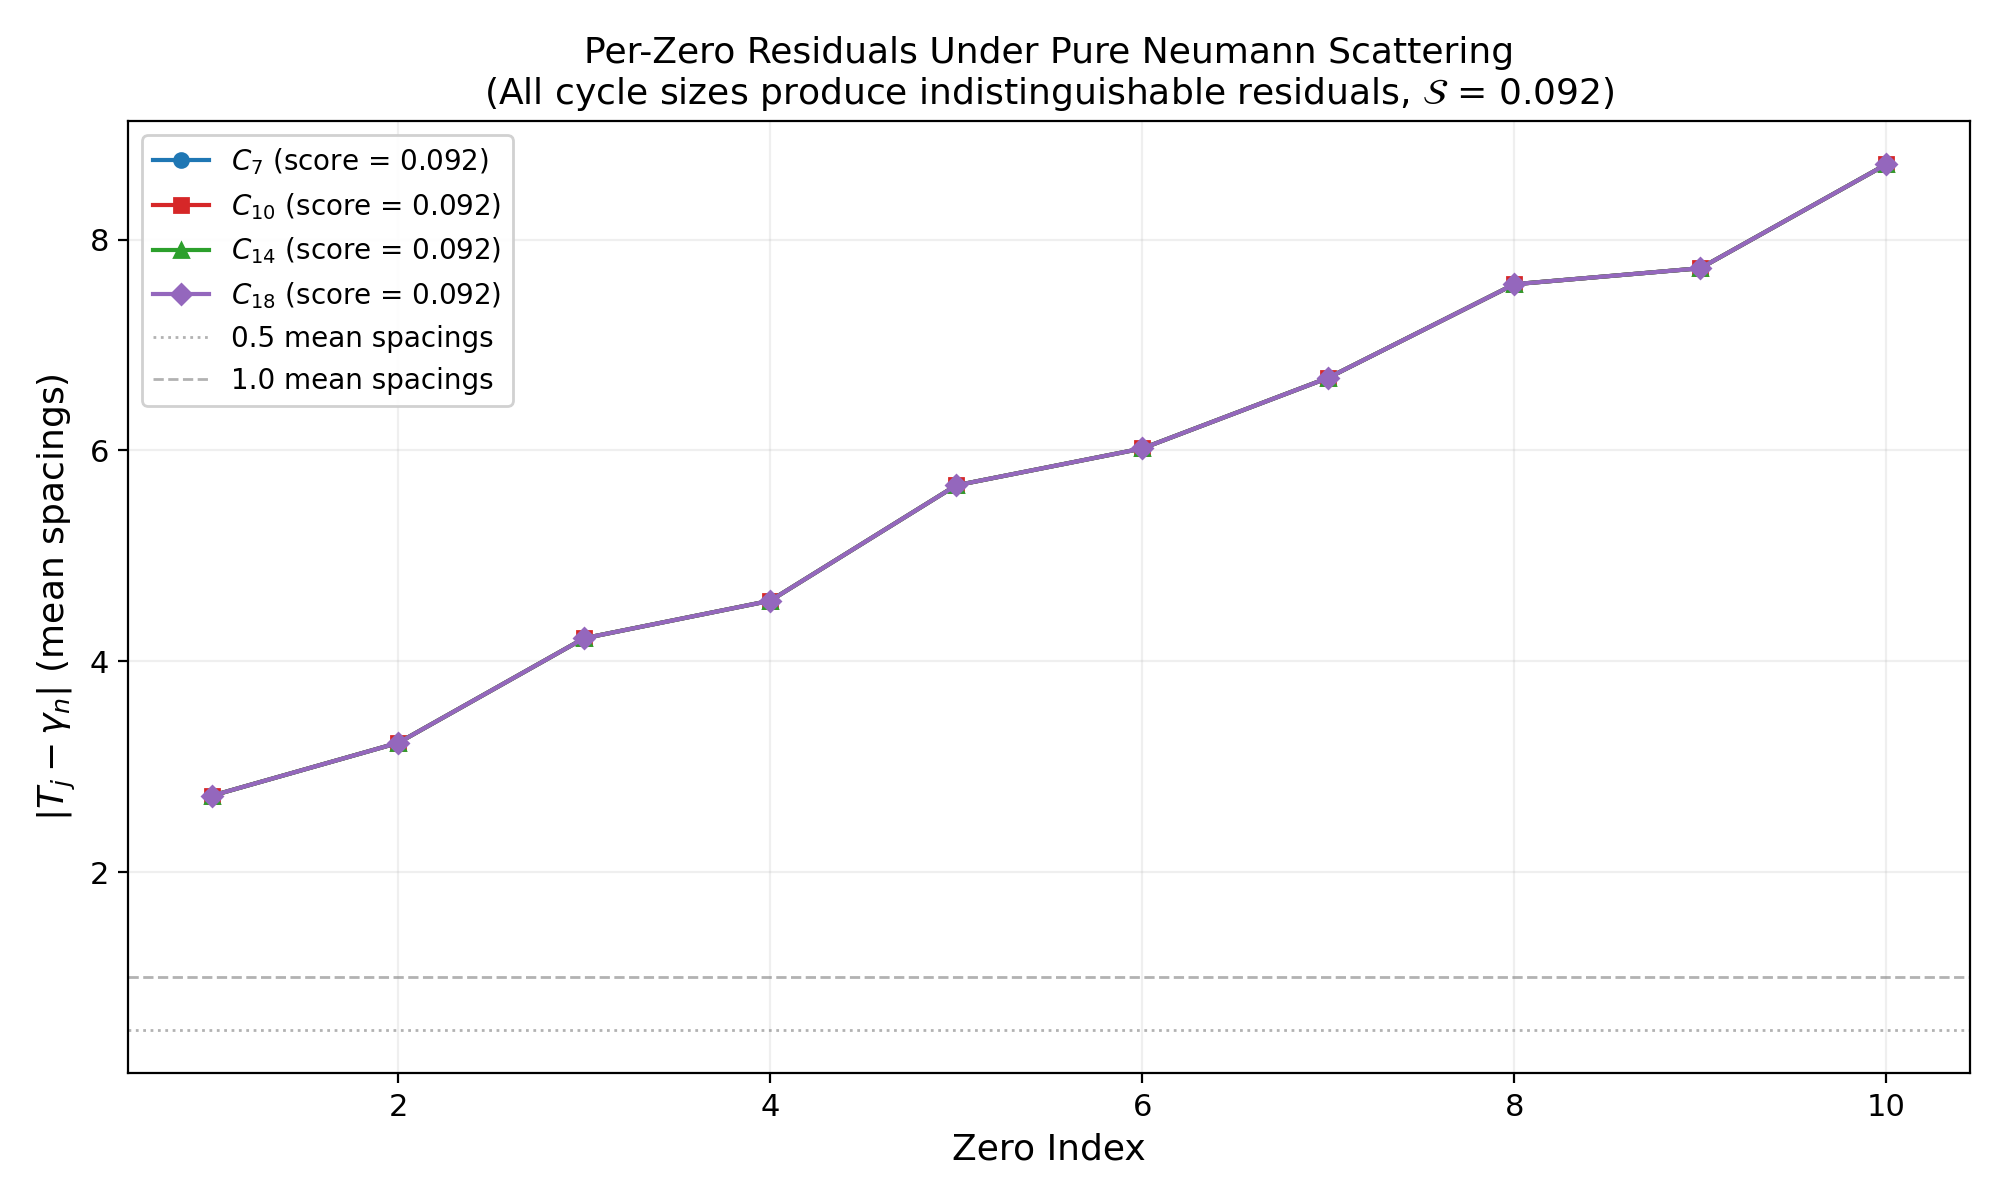
\includegraphics[width=\linewidth]{results/figure2_neumann_residuals.png}
\caption{Per-zero residuals $|T_j - \gamma_n|$ for cycle graphs $C_7$, $C_{10}$, $C_{14}$, $C_{18}$ under pure Neumann scattering, plotted against zero index. All four cycle sizes produce indistinguishable residuals (all $\mathcal{S} = 0.092$), confirming the size-independence of the Neumann ceiling. Dotted and dashed lines indicate residuals of $0.5$ and $1.0$ mean spacings respectively.}
\label{fig:neumannResiduals}
\end{figure}

\subsection{U(2) scattering on $C_7$}
\label{sec:results-U2}

Replacing Neumann conditions with full U(2) vertex scattering on $C_7$ --- introducing 4 real degrees of freedom per vertex while preserving self-adjointness of the graph Laplacian by construction~\cite{r3} --- yields a best score of $\mathcal{S} = 0.897$ against $100$ zeros, with MAD $= 0.145$ mean spacings. Across $30$ independent restarts from random initializations, the mean score is $0.884$ (std $0.006$), with every restart exceeding $\mathcal{S} = 0.87$. The improvement over the Neumann ceiling ($\Delta\mathcal{S} = +0.177$) is the largest single-step effect observed in this study.

The per-zero residual distribution is non-uniform: $74$ of $100$ zeros are matched to within $0.22$ mean spacings, and $25$ to within $0.045$ mean spacings, but $3$ zeros (indices $41$, $73$, $18$) have residuals exceeding $0.45$ mean spacings. The scattering matrices are far from Neumann (mean Frobenius distance $1.96$, on a scale of $[0, 2\sqrt{2}]$) with significant mean reflection probability $|r|^2 = 0.17$, compared to $0$ for pure Neumann transmission.

The monodromy matrix $M = \prod_v S_v$ exhibits a partial structure: $8$ of $30$ restarts produce a monodromy eigenvalue within $0.15$ of $-1$ (antiperiodic boundary conditions). These include the three highest-scoring solutions ($\mathcal{S} = 0.897, 0.893, 0.891$); the mean score for near-$(-1)$ restarts is $0.886$ versus $0.882$ for the remainder. However, the $-1$ eigenvalue is unstable under parameter perturbations as small as $\varepsilon = 10^{-4}$. Individual scattering matrices show no detectable number-theoretic structure: determinant phases are non-constant across vertices, and the near-$(-1)$ monodromy is a property of the composition, not of the individual matrices.

\subsection{Cycle-size scaling under U(2) scattering}
\label{sec:results-scaling}

Extending the joint optimization to cycle sizes $C_5$ through $C_{21}$, with $10$ random restarts per size and $7.5 \times 10^4$ evaluations per restart, reveals a slow improvement of correspondence with cycle size (Figure~\ref{fig:u2Scaling}). The best-score curve is non-monotonic: it climbs from $\mathcal{S} = 0.885$ at $C_5$ to a high of $\mathcal{S} = 0.9258$ at $C_{20}$, with intermediate dips at $C_8$, $C_{12}$, and $C_{14}$. These dips reflect optimization difficulty at higher parameter dimension (the parameter space grows as $5n$, reaching $100$ dimensions at $C_{20}$) rather than structural saturation: the mean-of-restarts score is the cleaner trend statistic and rises monotonically from $0.880$ at $C_5$ to $0.907 \pm 0.010$ at $C_{20}$, with $C_{21}$ at $0.902$ consistent within noise. A logarithmic fit $\mathcal{S}(n) = 0.023 \ln n + 0.849$ describes the mean trajectory with $R^2 = 0.84$.

\paragraph{Reproducibility of the $C_{20}$ best result.} The single highest-scoring graph in this study, $C_{20}$ at $\mathcal{S} = 0.9258$, requires careful interpretation. Re-scoring the saved parameters from scratch reproduces $\mathcal{S} = 0.92580628$ to 16-digit precision across five replicate scorings, with score sensitivity to spectrum sampling resolution of $\pm 0.0003$ across $n_{\mathrm{points}} \in \{1500, 8000\}$ --- confirming that the result is a mathematically valid score of the saved configuration. However, this graph was found in $1$ of $10$ random initializations during the cycle-size sweep, and $24$ subsequent CMA-ES restarts initialized in a Gaussian neighborhood ($\sigma_{\mathrm{edge}} = 0.3$, $\sigma_{\mathrm{scat}} = 0.5$) of these parameters failed to reach $\mathcal{S} = 0.9258$ --- the best refinement restart reached $\mathcal{S} = 0.9176$, with mean $0.902 \pm 0.008$. The $\mathcal{S} = 0.9258$ point therefore represents a narrow local optimum rather than the floor of a broad basin: a valid configuration whose existence we report, but not the typical outcome of optimization. The reproducible-by-optimization score at $C_{20}$ is $\mathcal{S} \approx 0.91$, with MAD $\approx 0.13$ mean spacings.

\begin{figure}[H]
\centering
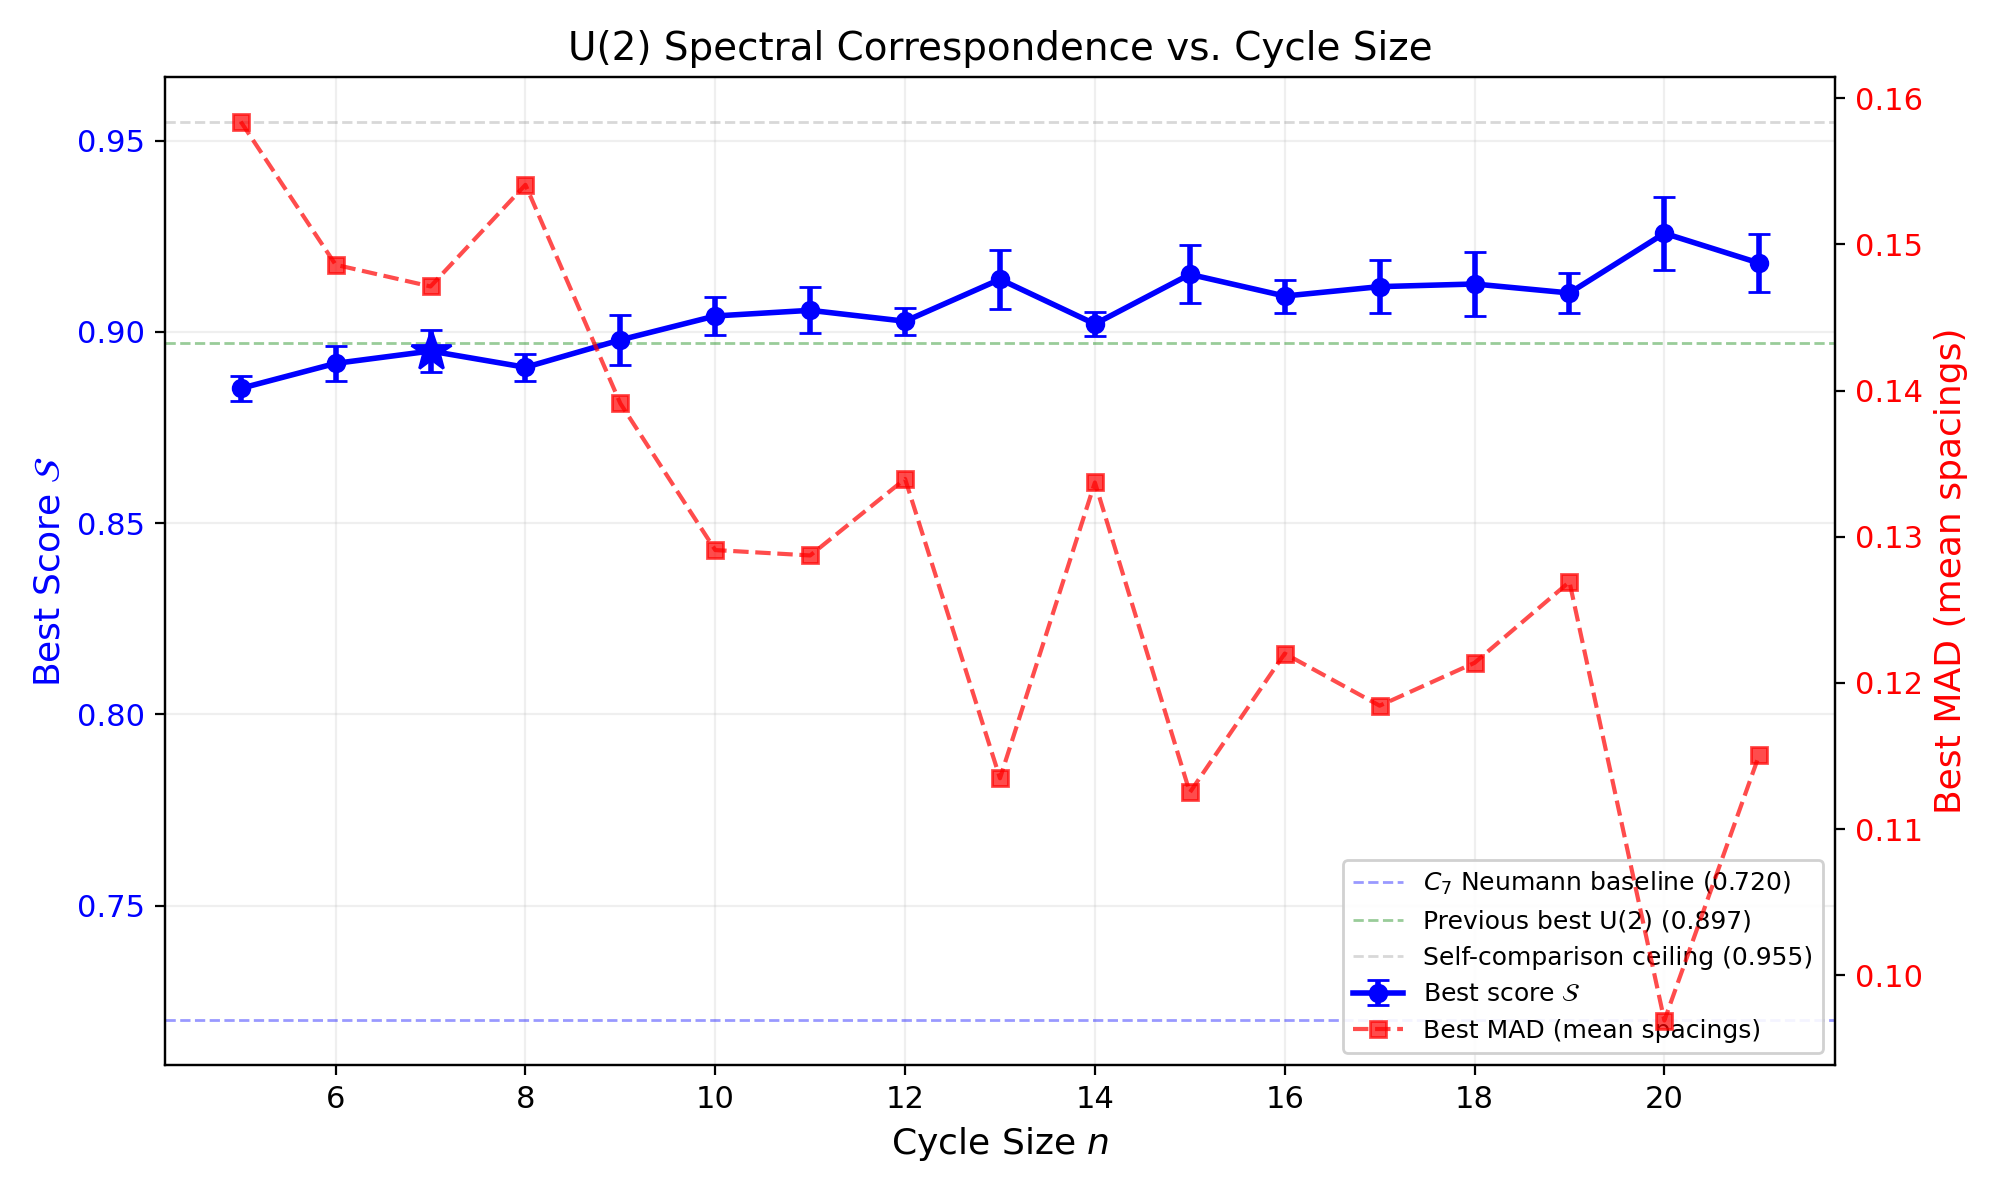
\includegraphics[width=\linewidth]{results/u2_scaling_plot.png}
\caption{Cycle-size scaling of best-of-restart score (left axis, blue) and best-of-restart MAD (right axis, red) under U(2) vertex scattering, across cycle sizes $C_5$ through $C_{21}$. Error bars on score show standard deviation across 10 restarts per size. Reference lines mark the $C_7$ Neumann ceiling ($0.720$), the original $C_7$ U(2) result ($0.897$), and the self-comparison ceiling ($0.955$).}
\label{fig:u2Scaling}
\end{figure}

\subsection{Topology independence under unitary scattering}
\label{sec:results-topology-indep}

To test whether the U(2) improvement is specific to the cycle topology, we performed analogous joint optimization on theta graphs $\Theta_k$ --- two degree-3 hub vertices connected by three paths of $k$ edges each --- for $k \in \{2, 3, 4, 5, 6\}$. The hubs carry full U(3) scattering (9 parameters each); internal degree-2 vertices carry U(2) scattering. Parameter counts range from $36$ at $k = 2$ ($5$ vertices, $6$ edges) to $96$ at $k = 6$ ($17$ vertices, $18$ edges), spanning the same range as the cycle sweep.

At every comparison point, the theta best and theta mean track the cycle to within $\pm 0.01$: at $k = 4$ ($66$D) theta best $0.9119$ vs cycle $C_{13}$ ($65$D) best $0.9138$; at $k = 5$ ($81$D) theta best $0.9078$ vs cycle $C_{16}$ ($80$D) best $0.9094$; at $k = 6$ ($96$D) theta best $0.9173$ vs cycle $C_{19}$ ($95$D) best $0.9102$. The theta mean of $0.9061$ at $k = 6$ slightly exceeds the cycle mean of $0.9011$ at $C_{19}$, providing weak evidence for a small advantage of degree-3 hubs at high parameter count, but the effect size ($\Delta\mathcal{S}_{\mathrm{mean}} \approx +0.005$) is within optimization noise.

We interpret this as evidence that graph topology is approximately irrelevant under unitary scattering, given matched parameter count. The relevant degree of freedom is the dimension of the unitary group at vertices --- equivalently, the number of independent boundary-condition parameters available to the optimizer --- not the connectivity structure of the graph. The improvement from Neumann to U(2) on $C_7$ ($\Delta\mathcal{S} = +0.18$) reflects the algebraic transition from a constrained two-parameter spectrum to a general $4n$-parameter scattering operator; the improvement from U(2) on $C_n$ to U(3)+U(2) on $\Theta_k$ at matched parameter count is small or absent.

\subsection{Algebraic structure of the optimal scattering data}
\label{sec:results-pslq}

To test whether the optimized scattering matrices possess hidden algebraic structure, we performed PSLQ integer-relation searches at $50$ decimal places on: the $28$ real and $28$ imaginary parts of the optimized U(2) matrix entries on the $C_7$ best graph; the $14$ eigenvalue phases of the U(2) matrices; the $7$ determinant phases; the $2$ monodromy eigenvalue phases; the $7$ optimized edge lengths; and the $28$ raw CMA-ES parameters $(\alpha_v, \beta_v, \gamma_v, \theta_v)$. We tested each value against bases including $\pi$, $\ln p$ for primes $p \leq 61$, $\sqrt{2}$, $\sqrt{3}$, $\sqrt{5}$, the golden ratio $\varphi$, and the Euler--Mascheroni constant $\gamma_E$, with maximum integer coefficient $|c| \leq 10$ and residual tolerance $10^{-20}$. Across all categories, zero integer relations were found. The optimal matrices and phases are numerically generic.

The only structural observation from the $C_7$ U(2) data is the near-$(-1)$ monodromy eigenvalue in 8 of 30 restarts, reported in Section~\ref{sec:results-U2}. This is a property of the matrix product around the cycle, not of any individual matrix or parameter. The eigenvalue is unstable under perturbation and absent in most high-scoring restarts (22 of 30); we report it as an observation warranting further investigation rather than an established structural result.

The PSLQ negative result is informative as a constraint on future analytic work: if a closed-form characterization of the optimal U(2) boundary conditions exists, it does not involve simple integer combinations of the natural mathematical constants at $50$ decimal places of precision. A more complex structure --- modular, elliptic, or involving special values of $L$-functions --- cannot be ruled out by this analysis.

\subsection{Riemann-specificity versus generic GUE alignment}
\label{sec:results-surrogate}

The U(2) correspondence at MAD $\approx 0.15$ mean spacings against the first $100$ Riemann zeros could in principle reflect either (i) a Riemann-specific structure in the optimal vertex conditions, or (ii) a generic capacity of U(2) cycle scattering to fit arbitrary GUE-distributed sequences of matched smooth density. The composite score weights GUE statistics (spacing distribution, pair correlation) at $0.30$, and by the Kottos--Smilansky theorem~\cite{r4} generic quantum graph spectra already satisfy GUE statistics; the load-bearing positional score $\mathcal{S}_{\mathrm{pos}}$ aligns two sequences both intrinsically GUE-distributed. The distinction between (i) and (ii) must therefore be established by direct control rather than by inspection of the score.

We performed this control by running the identical optimization pipeline against two matched sets of targets: $K = 50$ independent GUE surrogate target sequences (each generated as described below) and $K_R = 30$ independent restart seeds against the actual Riemann zeros. Both sets use the same $C_7$ topology, U(2) vertex scattering, CMA-ES with $5$ restarts and $7.5 \times 10^4$ evaluations per restart, and Nelder--Mead polish, so the two resulting MAD distributions are directly comparable. Each surrogate target is generated by (a) sampling eigenvalues of a $400 \times 400$ Gaussian Unitary Ensemble matrix, (b) taking the central $100$ eigenvalues for cleanest bulk statistics, (c) polynomial-unfolding to a staircase function, and (d) mapping back through $N_{\mathrm{smooth}}^{-1}$ so the surrogate's smooth counting density matches the Riemann--von Mangoldt density at the location of the first $100$ zeros. The resulting surrogate sequences possess GUE local statistics by construction (spacing coefficient of variation $0.45 \pm 0.05$, matching the Riemann value of $0.465$) and Riemann smooth counting density (mean spacing $2.21 \pm 0.04$, Riemann value $2.246$), with no Riemann arithmetic information.

The two distributions are strongly separated. Across the $K_R = 30$ Riemann seeds the pipeline reaches MAD $= 0.148 \pm 0.006$ mean spacings (mean $\pm$ standard deviation across seeds), with minimum $0.133$, maximum $0.159$, median $0.148$, and interquartile range $[0.143, 0.152]$. The corresponding score distribution is $\mathcal{S} = 0.892 \pm 0.004$. Across the $K = 50$ surrogates the pipeline reaches MAD $= 0.260 \pm 0.036$ mean spacings, with minimum $0.206$, maximum $0.377$, median $0.259$. Every one of the $30 \cdot 50 = 1500$ pairs $(r, s)$ of a Riemann-seed MAD $r$ and a surrogate MAD $s$ has $r < s$: the Riemann maximum ($0.159$) lies below the surrogate minimum ($0.206$), with a gap of approximately one Riemann standard deviation and one surrogate standard deviation between them. Every optimization on both sides matches all $100$ targets within the $\pm \Delta\gamma$ matching window ($M = 100$), so the two MAD distributions are computed on a common denominator and are directly comparable without a coverage confound.

A two-sided Mann--Whitney U test on the $K_R = 30$ Riemann MADs versus the $K = 50$ surrogate MADs yields $U = 0$ with exact $p \approx 2.3 \times 10^{-22}$ (SciPy's \texttt{mannwhitneyu} with \texttt{method="exact"}) and asymptotic $p \approx 9.4 \times 10^{-14}$; we report the exact value as primary. The corresponding effect size is Cliff's $|\delta| = 1.000$ with degenerate confidence interval, reflecting that every Riemann-seed MAD is strictly less than every surrogate MAD across all $30 \times 50 = 1500$ pairs. Under the standard exchangeability assumption of the test --- namely that Riemann and surrogate MADs are exchangeable draws from a common distribution under the null --- the observed distributional separation cannot be attributed to sampling variation across seeds. Both arms use the same $5$ CMA-ES restarts per experimental unit (Table~\ref{tab:experiment-map}) and the same optimization budget per restart, so the comparison is not confounded by unequal compute. Because every optimization on both sides matches all $100$ targets within the $\pm \Delta\gamma$ window ($M = N = 100$), the greedy sorted matching used in $\mathcal{S}_{\mathrm{pos}}$ coincides with the optimal-cost assignment on ordered sequences, and the reported MAD is invariant under alternative one-to-one pairings that respect the window. We do not claim that this test rules out every possible confounder: the two samples share the same optimizer, so any structural bias of the optimizer toward Riemann-shaped targets would appear as a distributional separation. What the test establishes is that generic GUE-density parameter richness at $5n = 35$ free parameters per configuration is not sufficient to explain the observed gap. Figure~\ref{fig:surrogateHist} shows the two distributions overlaid.

We interpret this as direct evidence that the U(2) cycle construction is not a generic spectral fitter for GUE-density targets: at $35$ free parameters, the pipeline reproducibly fits the Riemann zeros to MAD $\approx 0.15$ across seeds but cannot fit any of $50$ independently drawn GUE-density targets below MAD $\approx 0.20$ at the same optimization budget. The construction finds structure specific to the Riemann zeros. What that structure is remains open: the PSLQ analysis of Section~\ref{sec:results-pslq} establishes that whatever structure is present is not visible as integer relations at $50$ decimal places against simple bases, and the surrogate control establishes only that its existence is empirically required by the distributional separation --- not that the finite-graph spectra converge to the Riemann zeros in any $n \to \infty$ limit. That stronger claim remains open.

{\sloppy All Riemann-seed and surrogate optimization records and aggregate statistics are deposited in the files \texttt{riemann\_seed\_distribution.jsonl}, \texttt{gue\_surrogate\_control.jsonl}, and their associated summary JSON files under \texttt{results/} in the public repository.\par}

\begin{figure}[H]
\centering
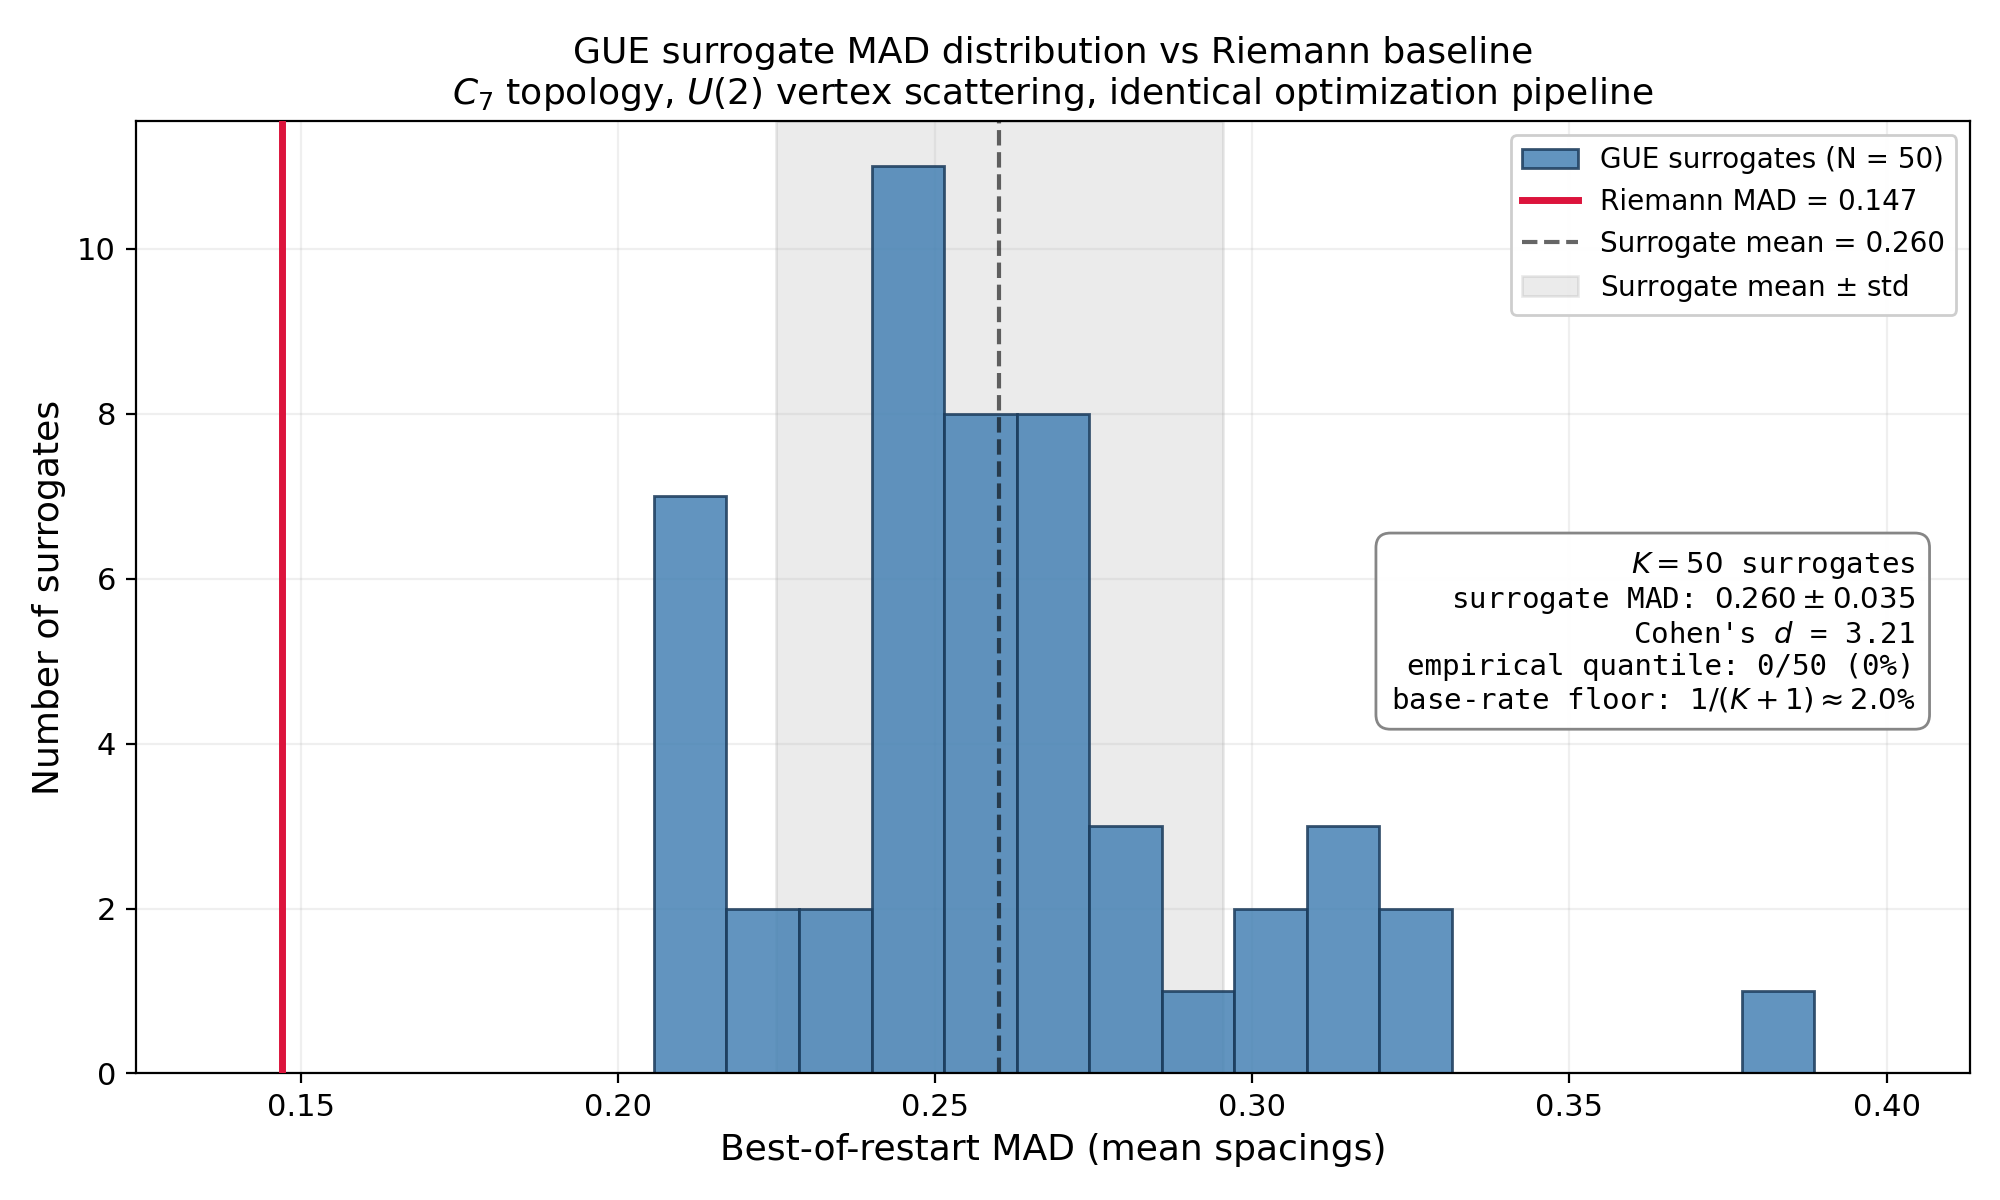
\includegraphics[width=\linewidth]{results/figure4_surrogate_distribution.png}
\caption{Riemann-seed and GUE-surrogate MAD distributions under the identical $C_7$ / U(2) CMA-ES + Nelder--Mead pipeline. Red: $K_R = 30$ independent Riemann-seed optimizations, MAD $= 0.148 \pm 0.006$. Blue: $K = 50$ independent GUE surrogate optimizations unfolded to the Riemann--von Mangoldt smooth density, MAD $= 0.260 \pm 0.036$. Dashed lines: distribution medians. The two distributions are disjoint (the Riemann maximum $0.159$ lies below the surrogate minimum $0.206$); every optimization on both sides matches all $100$ targets within the matching window, so the separation is carried entirely by positional accuracy on matched targets. Two-sided Mann--Whitney $U = 0$, exact $p \approx 2.3 \times 10^{-22}$; Cliff's $|\delta| = 1.000$.}
\label{fig:surrogateHist}
\end{figure}

\subsection{Reflection-magnitude ablation}
\label{sec:results-reflection}

Remark~\ref{rem:reflection} identifies the reflection magnitude $|\cos\theta_v|$ at degree-$2$ vertices as the algebraic property distinguishing the Neumann/TRS-broken family (reflectionless, $S_{ii} = 0$) from the general U(2) family. That identification is algebraic; whether reflection magnitude quantitatively drives the observed ceiling-breaking is an empirical question that Remark~\ref{rem:reflection} alone does not settle. We tested it directly.

For each of $12$ fixed values of $\theta_v$ on a uniform grid $[0.05, \pi/2 - 0.05]$ (twelve values sampling $|\cos\theta_v|$ from $0.999$ down to $0.050$), we ran the identical CMA-ES + Nelder--Mead pipeline against the first $100$ Riemann zeros, holding $\theta_v$ fixed at every vertex of $C_7$ and freely optimizing over the remaining $3n$ scattering phases $(\alpha_v, \beta_v, \gamma_v)$ and $n$ edge lengths (total $4n = 28$ parameters versus the $5n = 35$ of the free U(2) case). Figure~\ref{fig:reflectionCurve} shows the resulting curve.

The curve is a clear inverted U. Both extremes collapse to $\mathcal{S} \approx 0.73$ (MAD $\approx 0.21$--$0.43$): at $|\cos\theta_v| \to 1$ the operator becomes progressively decoupled at each vertex and the graph fragments into disjoint edges, and at $|\cos\theta_v| \to 0$ the constraint $S_{ii} = 0$ forces something close to the TRS-broken Neumann family whose ceiling is $\mathcal{S} \approx 0.72$. In between, the peak sits at $|\cos\theta_v| \approx 0.55$ with $\mathcal{S} = 0.886$, MAD $= 0.155$. Three qualitative consequences.

First, reflection is necessary: even with the full $(\alpha, \beta, \gamma)$ phase freedom at every vertex, imposing reflectionlessness ($|\cos\theta_v| \to 0$) prevents the operator from exceeding a score close to the TRS-broken Neumann ceiling. This confirms the mechanistic claim of Remark~\ref{rem:reflection} in the direction it was made.

Second, reflection is not by itself sufficient: fully reflecting scattering ($|\cos\theta_v| \to 1$) fragments the graph and hits the same low ceiling. The improvement from Neumann to full U(2) is not obtained by pushing reflection arbitrarily high.

Third, the sweet spot at $|\cos\theta_v| \approx 0.55$ is a quantitative and testable prediction of the construction: at this specific reflection amplitude the operator has just enough vertex-level decoupling to escape the reflectionless family while retaining enough connectivity to support extended eigenmodes across the cycle. Whether the position of this peak is special to the Riemann targets or is a generic feature of U(2) cycle scattering against any GUE-density sequence is a natural next question for the ablation--surrogate combination.

\begin{figure}[H]
\centering
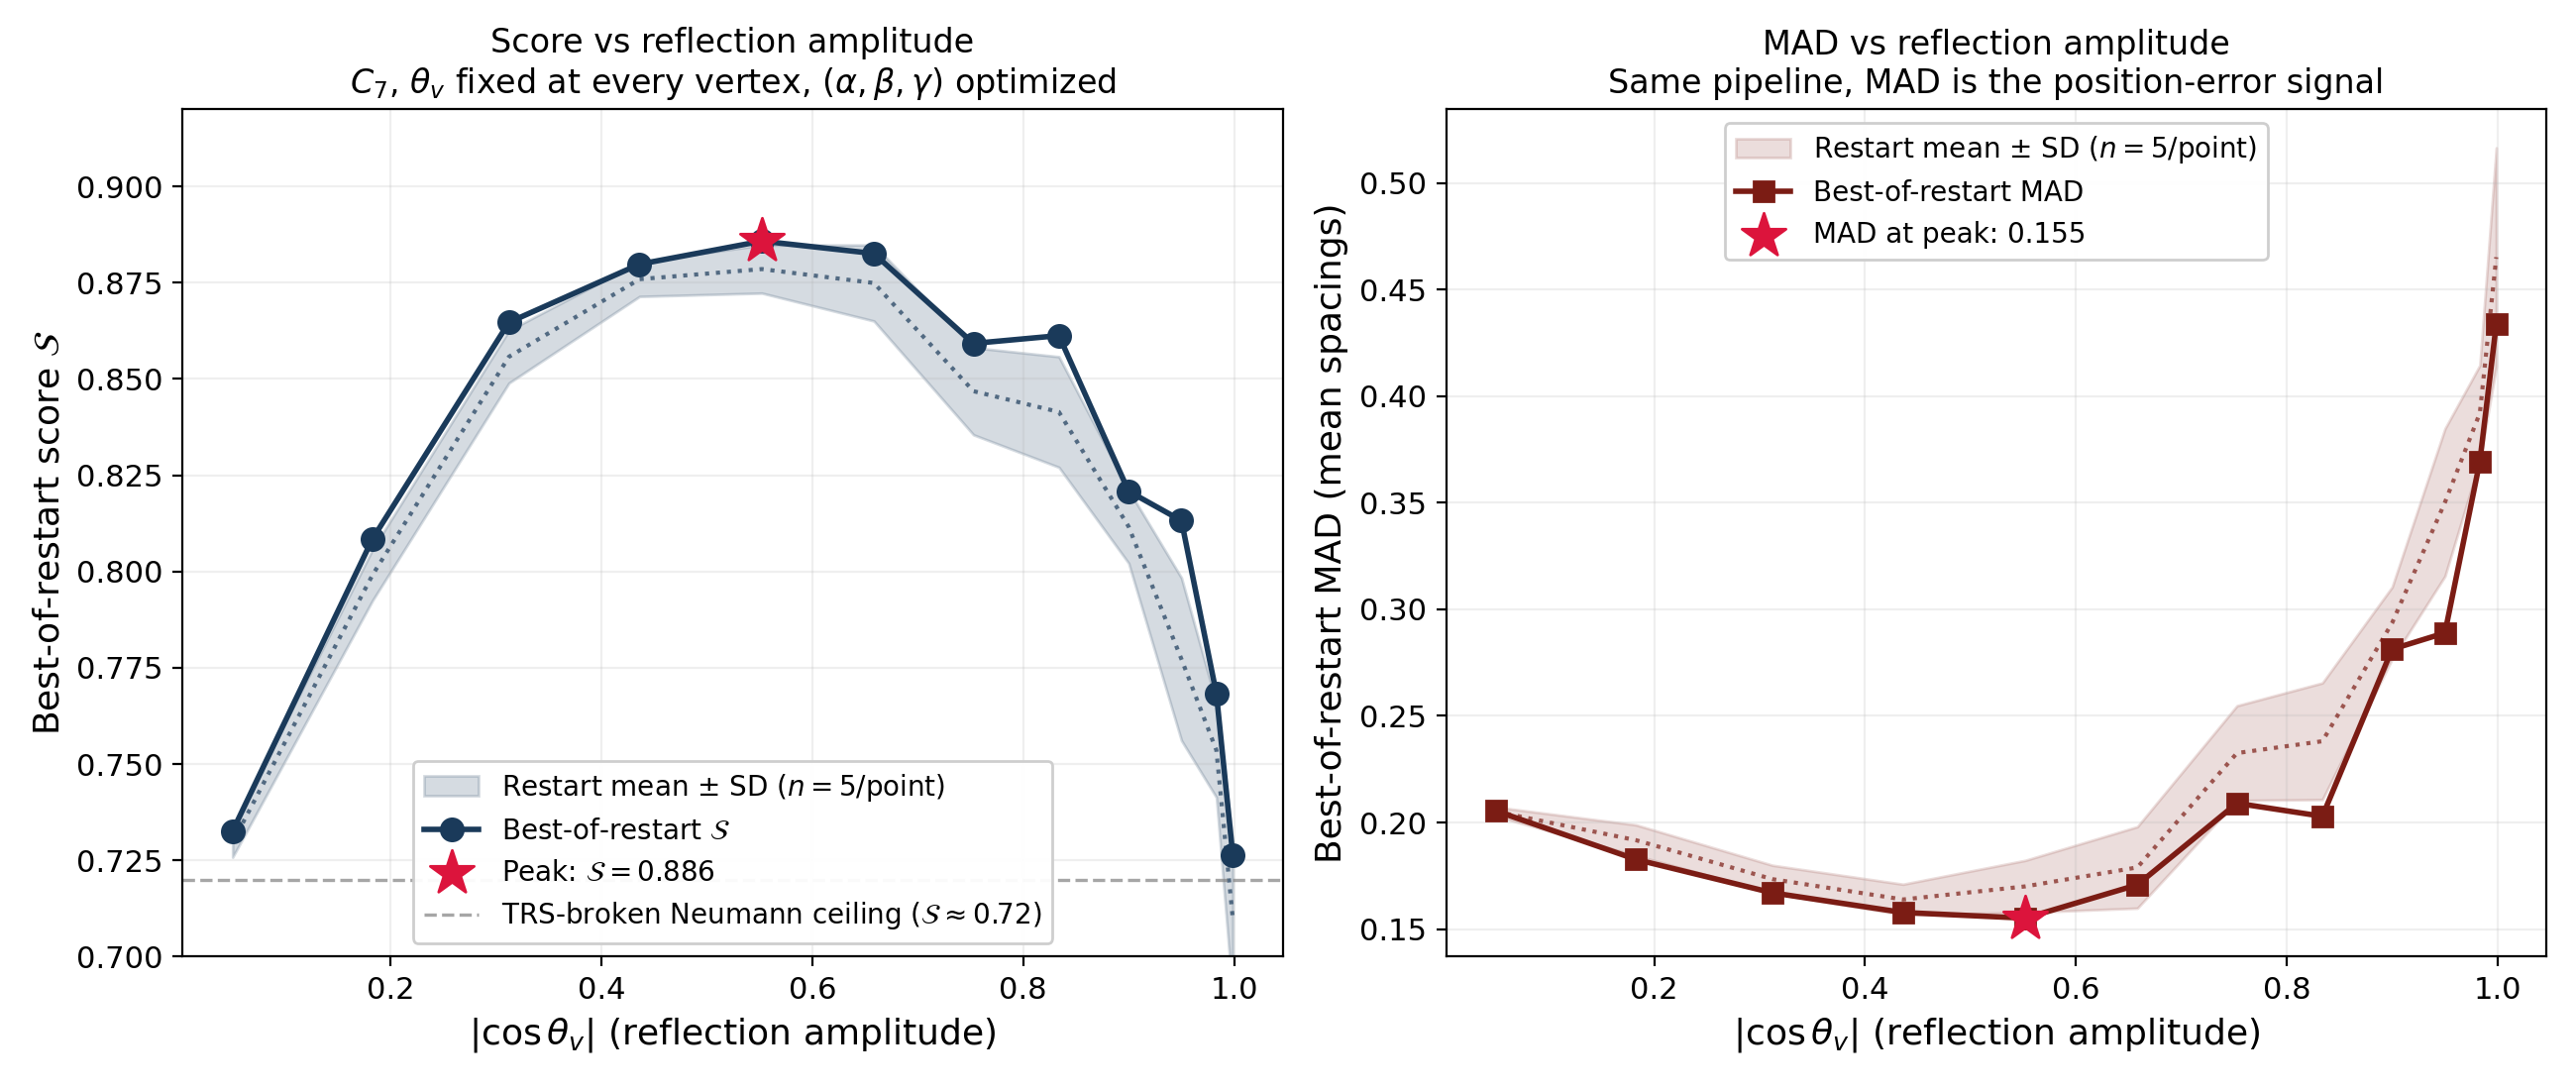
\includegraphics[width=\linewidth]{results/figure5_reflection_curve.png}
\caption{Reflection-magnitude ablation. Best-of-restart score $\mathcal{S}$ (left) and best-of-restart MAD (right) versus the fixed reflection amplitude $|\cos\theta_v|$ at every vertex, with $(\alpha_v, \beta_v, \gamma_v)$ and edge lengths optimized. Twelve $\theta_v$ values sample $|\cos\theta_v|$ from $0.999$ (near-fully reflecting) to $0.050$ (near-reflectionless). Solid curves: best of $5$ restarts per $\theta_v$. Shaded bands: restart mean $\pm$ standard deviation across the $5$ restarts, showing that the inverted-U shape is well outside restart-level optimization noise ($\mathcal{S}$-band width $\sim 0.01$ near the peak versus a $\mathcal{S}$ excursion of $\sim 0.16$ from peak to either extreme). The curve peaks at $|\cos\theta_v| \approx 0.55$ with $\mathcal{S} = 0.886$, MAD $= 0.155$; both extremes collapse to $\mathcal{S} \approx 0.73$. Dashed gray line (left): the TRS-broken Neumann ceiling at $\mathcal{S} \approx 0.72$ for reference.}
\label{fig:reflectionCurve}
\end{figure}

%% =====================================================================
\section{Discussion}
\label{sec:discussion}

\subsection{The conceptual inversion}
\label{sec:disc-inversion}

The dominant axis of improvement in spectral correspondence under our framework is the vertex scattering condition, not edge-length geometry. Replacing Neumann boundary conditions with general U(2) matrices while keeping the simplest possible topology ($C_7$) produces the largest score improvement observed ($\Delta\mathcal{S} = +0.177$). The mechanism identified algebraically in Remark~\ref{rem:reflection} and tested directly in Section~\ref{sec:results-reflection} is more specific than ``general U(2) freedom.'' Neumann and TRS-broken Neumann scattering at degree-2 vertices are both reflectionless, and the transition to nonzero reflection magnitude $|\cos\theta_v| > 0$ is required to break the rigid $(L, \Phi)$ family: even with the full $(\alpha, \beta, \gamma)$ phase freedom of U(2) at every vertex, the reflectionless limit collapses back to a score close to the TRS-broken Neumann ceiling of $0.72$. Reflection is genuinely doing work; the additional phase parameters of U(2) at reflectionless scattering are not by themselves enough to break the ceiling. The reflection-magnitude ablation (Figure~\ref{fig:reflectionCurve}) refines this picture in one direction the algebraic argument did not anticipate: reflection is necessary but not monotonically good. There is an interior optimum at $|\cos\theta_v| \approx 0.55$ where the operator has just enough vertex decoupling to escape the reflectionless family while retaining enough connectivity to support extended eigenmodes; past the optimum, further reflection progressively decouples the graph and score falls back. The mechanistic conclusion is therefore that the arithmetic --- to the extent it is represented at all --- lives at the junctions in the reflection magnitude, and specifically at a moderate value of it. Exhaustive variation of topology and edge lengths under Neumann conditions yields at most $\Delta\mathcal{S} \approx +0.08$ above the random-spectrum floor. Variation of graph topology under U(2) scattering (cycle vs theta at matched parameter count) yields at most $\pm 0.01$ in best-of-restart $\mathcal{S}$ across the tested parameter counts. The graph is scaffolding; the arithmetic lives at the junctions. This conclusion is at odds with the dominant intuition in the quantum-graph approach to the Riemann zeros since at least Berry and Keating~\cite{r5}, which has typically anticipated that edge lengths proportional to logarithms of primes would encode the arithmetic information via the trace formula. The ``primes in the wires'' expectation does not survive the data under the reflectionless-Neumann search space and U(2) budgets we explored; whether it can be rescued under alternative parameterizations we did not test remains open.

\subsection{Convergence behavior under cycle-size scaling}
\label{sec:disc-convergence}

Under U(2) scattering, the mean score across optimization restarts increases logarithmically with cycle size, from $0.880$ at $C_5$ to $0.907$ at $C_{20}$. The empirical fit $\mathcal{S}(n) = 0.023 \ln n + 0.849$ with $R^2 = 0.84$ describes the available data but cannot be extrapolated reliably. A naive extrapolation to $\mathcal{S} = 0.955$ (the self-comparison ceiling) would require $n \sim 100$, but the optimization difficulty at $n = 100$ ($5n = 500$ dimensions) is severe enough that CMA-ES with current budgets would likely fail to find such solutions even if they exist. Whether the underlying mathematical limit of U(2)-on-cycle correspondence approaches $0.955$, plateaus at some intermediate value, or is bounded by some structural obstacle we have not identified, cannot be settled by the present data. We emphasize the distinction between best-of-restart and mean-of-restart statistics. The $C_{20}$ best of $0.9258$ is a verified-reproducible-by-evaluation result that arose in $1$ of $10$ random restarts and was not reproduced from $24$ subsequent Gaussian-neighborhood restarts. The mean across all $10$ restarts at $C_{20}$ is $0.907$. The honest summary is that finite quantum graphs under U(2) vertex scattering achieve correspondence with the first $100$ Riemann zeros at MAD between $0.10$ and $0.15$ mean spacings depending on optimization budget, with the lower end of this range representing fragile local optima rather than broad attractors.

\subsection{Comparison to prior work}
\label{sec:disc-prior}

Bender, Brody, and M\"uller~\cite{r12} construct a non-Hermitian Hamiltonian whose eigenvalues, by formal manipulation of operator identities, correspond to the Riemann zeros. The self-adjointness of the resulting operator depends on a choice of boundary condition whose validity remains open. The quantum-graph Laplacian here is self-adjoint by construction under U(2) vertex conditions~\cite{r3}, removing this concern in the graph setting, and yields a measurable spectral deviation of MAD $\approx 0.10$--$0.15$ mean spacings against $100$ zeros --- a quantitative benchmark we believe to be novel for this construction class. Creffield and Sierra~\cite{r13} demonstrate a Floquet-driven cold-atom system whose quasi-energies are engineered to reproduce the first $80$ zeros, with the drive phases chosen explicitly to encode the zero sequence. The present result differs in that no such construction is imposed: the U(2) parameters are optimized freely from random initializations, and the correspondence emerges from the optimization. This makes the present work a discovery (the optimizer finds high-correspondence configurations that were not put in by hand) rather than a verification of a designed correspondence. LeClair and Mussardo~\cite{r6} develop generalized Euler-product constructions whose zeros formally correspond to the Riemann zeros via analytic continuation; the present construction is unrelated except in spirit, both being attempts to realize the Hilbert--P\'olya idea in a self-adjoint setting. Schumayer and Hutchinson~\cite{r8} provide a colloquium-level review of physical approaches to the Riemann hypothesis; we view the present work as a contribution to the methodological landscape they survey.

\subsection{The monodromy observation}
\label{sec:disc-monodromy}

The appearance of a near-$(-1)$ monodromy eigenvalue in $8$ of $30$ high-scoring $C_7$ U(2) restarts corresponds physically to antiperiodic (fermionic) boundary conditions around the cycle. It connects suggestively to the functional equation $\zeta(s) = \chi(s)\,\zeta(1-s)$, which encodes the symmetry $s \to 1 - s$ of the critical strip --- the same symmetry whose fermionic analogue is antiperiodic boundary conditions on a closed path. The fragility of this eigenvalue under parameter perturbations as small as $\varepsilon = 10^{-4}$, however, and its absence in the cycle-size sweep results at $C_n$ for $n \geq 7$ (zero of the $17$ best-of-restart results from $C_5$ through $C_{21}$ exhibit near-$(-1)$ monodromy), indicate that it is not a necessary condition for spectral correspondence. We report it as an observation warranting further investigation rather than an established structural result. A targeted study of whether constraining the monodromy to exactly $-I$ during optimization improves correspondence is a natural next experiment.

\subsection{The PSLQ negative result}
\label{sec:disc-pslq}

The absence of integer relations at $50$ decimal places against natural mathematical-constant bases is informative as a constraint on the form an analytic characterization could take. If a closed-form expression for the optimal U(2) vertex conditions exists, it does not reduce to simple linear or quadratic combinations of $\pi$, $\ln p$, square roots, or the standard transcendental constants. The optimal data could still possess structure detectable by methods we did not apply --- modular relations, elliptic-curve parameterizations, special values of $L$-functions, or relations at higher PSLQ precision against larger bases --- or it could be genuinely generic, in which case the spectral correspondence is a property of the joint configuration space rather than of any individually distinguished point in it. We note that this negative result is methodologically valuable for the broader research program: future computational searches for Hilbert--P\'olya-type operators on quantum graphs need not waste effort searching for simple closed-form vertex conditions at $50$ dp.

\subsection{Open questions}
\label{sec:disc-open}

The present work suggests the following directions, in increasing order of difficulty:
\begin{enumerate}
    \item \textbf{Higher-dimensional unitary scattering.} U($d$) at degree-$d$ vertices for $d \geq 3$ has been tested only on theta graphs (U(3) at hubs) at modest sizes. A degree sweep using complete graphs $K_n$ --- with U($n-1$) at every vertex --- would test whether the small advantage observed for U(3) over U(2) at matched parameter count continues to higher degree, or whether the correspondence saturates as a function of unitary dimension.
    \item \textbf{Modular and elliptic structure searches.} PSLQ at $50$ dp tests linear relations against fixed bases; the optimal scattering data could possess modular-form or elliptic-curve structure invisible to this test. A systematic search using LLL reduction against bases of $L$-function special values, modular invariants, and class-field-theoretic constants is feasible at the precision of the saved parameters.
    \item \textbf{Analytic characterization.} The strongest version of the open question is whether the optimal vertex conditions admit a closed-form characterization at all. The negative PSLQ result rules out simple forms; the discovery of any analytic expression for the $C_n$ U(2) optimal vertex conditions, if such an expression exists, would constitute a major mathematical advance, and would by construction yield a self-adjoint operator whose spectrum approximates the Riemann zeros analytically.
\end{enumerate}

We do not claim to have made progress on the Riemann hypothesis itself. What we have identified is a numerical and methodological target for the Hilbert--P\'olya program: the construction class consists of cycle or theta graphs with full U($d$) vertex scattering; the optimization landscape is rugged but admits configurations at MAD $\sim 0.10$ mean spacings; the relevant structure lives at the vertices, not in the edge geometry; the structure, if analytic, is not visible at $50$ decimal places of precision against simple bases; and the structure is empirically specific to the Riemann zeros, not generic to matched-density GUE targets. The present result identifies the target and characterizes its empirical properties; finding the analytic characterization, if one exists, is the remaining step.

%% =====================================================================
\section*{Acknowledgements}

Computational experiments were implemented with assistance from Claude Code (Anthropic) for software development and analysis scripting. Scientific interpretation, framing, and conclusions are the author's.

\section*{Conflicts of Interest}

The author declares no competing financial interests.

\section*{Funding}

This research received no specific grant from any funding agency in the public, commercial, or not-for-profit sectors.

\section*{Data Availability}

{\sloppy All code, optimization results, the Theorem~\ref{thm:neumann} proof, the five manuscript figures, the complete $K = 50$ GUE surrogate data deposit, the $K_R = 30$ Riemann-seed distribution deposit, and the reflection-magnitude ablation deposit are publicly available at \url{https://github.com/photodoc1960/Riemann-quantum-graph}. The three JSONL deposits and their associated summary JSON files are located under \texttt{results/}.\par}

%% =====================================================================
%%  Bibliography
%%
%%  Pre-submission TODO: add MathSciNet IDs via \MR{xxxxxxx} where available
%%  by looking up each entry on mathscinet.ams.org.

\begin{thebibliography}{99}

\bibitem{r1}
H. L. Montgomery,
The pair correlation of zeros of the zeta function,
\textit{Proc. Symp. Pure Math.} \textbf{24} (1973), 181--193.
% MR: TBD

\bibitem{r2}
A. M. Odlyzko,
On the distribution of spacings between zeros of the zeta function,
\textit{Math. Comp.} \textbf{48} (1987), 273--308.
% MR: TBD

\bibitem{r3}
V. Kostrykin and R. Schrader,
Kirchhoff's rule for quantum wires,
\textit{J. Phys. A} \textbf{32} (1999), 595--630.
% MR: TBD

\bibitem{r4}
T. Kottos and U. Smilansky,
Periodic orbit theory and spectral statistics for quantum graphs,
\textit{Ann. Phys.} \textbf{274} (1999), 76--124.
% MR: TBD

\bibitem{r5}
M. V. Berry and J. P. Keating,
The Riemann zeros and eigenvalue asymptotics,
\textit{SIAM Rev.} \textbf{41} (1999), 236--266.
% MR: TBD

\bibitem{r6}
A. LeClair and G. Mussardo,
Generalized Riemann hypothesis, time series and normal distributions,
\textit{J. Stat. Mech.} \textbf{2019} (2019), 023203.
% MR: TBD

\bibitem{r7}
M. Sieber and K. Richter,
Correlations between periodic orbits and their r\^ole in spectral statistics,
\textit{Phys. Scr.} \textbf{T90} (2001), 128--133.
% MR: TBD

\bibitem{r8}
D. Schumayer and D. A. W. Hutchinson,
Colloquium: Physics of the Riemann hypothesis,
\textit{Rev. Mod. Phys.} \textbf{83} (2011), 307--330.
% MR: TBD

\bibitem{r9}
H.~M. Edwards,
\textit{Riemann's Zeta Function},
Academic Press, New York (1974),
Appendix (English translation of B. Riemann,
``\"Uber die Anzahl der Primzahlen unter einer gegebenen Gr\"osse,''
Monatsberichte der Berliner Akademie, November 1859).
% MR: MR0466039

\bibitem{r10}
G. Berkolaiko and P. Kuchment,
\textit{Introduction to Quantum Graphs},
American Mathematical Society, Providence, RI (2013).
% MR: MR3013208

\bibitem{r11}
N. Hansen,
The CMA evolution strategy: A tutorial,
in \textit{Towards a New Evolutionary Computation}, edited by J. A. Lozano et al.,
Springer (2006), pp. 75--102.
% MR: N/A (book chapter)

\bibitem{r12}
C. M. Bender, B. K. Brody, and M. P. M\"uller,
Hamiltonian for the zeros of the Riemann zeta function,
\textit{Phys. Rev. Lett.} \textbf{118} (2017), 130201.
% MR: TBD

\bibitem{r13}
C. E. Creffield and G. Sierra,
Finding zeros of the Riemann zeta function by periodic driving of cold atoms,
\textit{Phys. Rev. A} \textbf{91} (2015), 063608.
% MR: TBD

\end{thebibliography}

\end{document}
